% !TEX encoding = UTF-8 Unicode
\documentclass[letterpaper,11pt, oneside]{layout}

%%%%%%%%%%%%%%%%%%%%%%%%%%%%%%%%%%%%%%%%%%%%%%%%
%%%%%%%%%%%%%%%%%%%% Title of Titlepage %%%%%%%%%%%%%%%%%%%%
%%%%%%%%%%%%%%%%%%%%%%%%%%%%%%%%%%%%%%%%%%%%%%%%

\title{Risk Calculation System}
\subtitle{MATH 5320 Financial Risk Management and Regulation Final Project}
\date{\today}

%%%%%%%%%%%%%%%%%%%%%%%%%%%%%%%%%%%%%%%%%%%%%%
%%%%%%%%%%%%%%%%%%%% Document %%%%%%%%%%%%%%%%%%%%
%%%%%%%%%%%%%%%%%%%%%%%%%%%%%%%%%%%%%%%%%%%%%%

\begin{document}
\cleardoublepage
\maketitle

\frontmatter
\begin{spacing}{1}
%\include{body/abstract}

\tableofcontents
\listoffigures
\listoftables
\end{spacing}

%%%%%%%%%%%%%%%%%%%%%%%%%%%%%%%%%%%%%%%%%%%%%%

\mainmatter

\chapter{Executive Summary}
\label{chap:summ}


This is a review of our group’s project of development of a risk calculation system for a user-defined portfolio. This system is used to calculate historical VaR and ES, parametric VaR and ES, as well as Monte Carlo VaR and ES.

The Model description is on Page 4, the current  model usage is on Page 7. Validation methodology and scope is on Page 8 and critical analysis is on Page 4.
%%%%%%%%%%%%%%%%%%%%%%%%%%%%%%%%%%%%%%%%%%%%%%

\begingroup
\renewcommand{\clearpage}{}
\chapter{Introduction}
\label{chap:intro}
\endgroup
This is a review of our group’s project of development of a risk calculation system for a portfolio comprised of stocks and options. In this system we realized the computation and visualization of historical VaR, GBM VaR, as well as VaR using Monte Carlo Simulation. 

The data we obtained for input is the historical Close Price daily for the stocks that user wants to form a portfolio. And our system do a calculation of VaR using historical simulation, parametric method, as well as Monte Carlo simulation.


%%%%%%%%%%%%%%%%%%%%%%%%%%%%%%%%%%%%%%%%%%%%%%

\begingroup
\renewcommand{\clearpage}{}
\chapter{Product Description}
\label{chap:pd}
\endgroup


Risk in stock and option investments is all about what might cause you to lose money on those investments. There are six main types of risk: inflation risk, interest rate risk, market risk, credit risk, liquidity risk and event risk. But their varying components can be interrelated. For example, a rise in inflation limits consumer buying power, so the Federal Reserve raises interest rates to curb inflation. Higher interest rates might weaken a company's ability to sell products and borrow funds inexpensively to finance its operations without losing money. 

In this report, we mainly focus on the market risk, which refers to the functioning of the marketplace. For stocks, they are exposed to the price changes, and for options, they have one more risk factor: the volatility.



%%%%%%%%%%%%%%%%%%%%%%%%%%%%%%%%%%%%%%%%%%%%%%

\begingroup
\renewcommand{\clearpage}{}
\chapter{Model Description}
\label{chap:md}
\endgroup

%%%%%%%%%%%%%%%%%%%%%%%%%%
\section{Modeling theory/assumptions}
\label{sec:md:mt}

We need to show what is Brownian Motion before we actually dig into Geometric Brownian Motion.

In mathematics, Brownian motion is described by the Wiener process; a continuous-time stochastic process named in honor of Norbert Wiener. It is one of the best known Levy processes (cadlag stochastic processes with stationary 
independent
increments) and occurs frequently in pure and applied mathematics, economics and physics.

The Wiener process Wt is characterized by four facts:

\begin{enumerate}
\item $W_0=0$
\item $W_t$ is almost surely continuous
\item $W_t$ has independent increments
\item $W_t-W_s\sim \mathcal{N}(0,t-s)$ for $0\le s\le t$
\end{enumerate}

A geometric Brownian Motion (GBM) (also known as exponential Brownian motion) is a continuous-time stochastic process in which the logarithm of the randomly varying quantity follows a Brownian motion (also called a Wiener process) with drift. It is an important example of stochastic processes satisfying a stochastic differential equation (SDE); in particular, it is used in mathematical finance to model stock prices in the Black–Scholes model. 

So in our risk calculation system, we are assuming any stocks and any portfolios consisting of only stocks (without options) resemble GBM. We use stocks/portfolios’ historical Closing Price for calibration in order to get the drift and volatility of the GBM model. To do this, we choose an appropriate window size, for instance, 2 years window, and then use the steps as follows to obtain the parameters of the GBM daily. 

\[\text{Log return}=\log(S_t/S_{t-1})\]
\[dt=\text{horizon (in days)}/252\]
\[\bar{\mu}=\text{mean}(\sqrt{\text{Log return}}-\sqrt{\text{Average}})\]
\[\bar{\sigma}=\sqrt{\bar{var}}, \quad \sigma=\bar{\sigma}/\sqrt{dt}\]
\[\mu=\bar{\mu}/dt+\sigma^2/2\]

So when calculating GBM VaR, we just input the parameters to the GBM Value-at-Risk Formula: 
\begin{equation}
VaR(S, T, p)=S_0-S_0 e^{\sigma\sqrt{T}\Phi^{-1}(1-p)+ (\mu-\frac{\sigma^2}{2})T}
\end{equation}

And we can easily get the GBM VaR for a certain period easily.


There are clearly some pros with this method:

Pros: 
\begin{itemize}
\item Only need to do the calculation of mu and sigma
\item the data for the input is easy to obtain
\end{itemize}

But still it has some drawback:
\begin{itemize}
\item the assumption of normality might be fatal
\item the data for the input is easy to obtain
\end{itemize}

Another method that directly make a normal assumption is Monte Carlo Simulation.

We can create simulation paths in two different ways: 
\begin{enumerate}
\item Form the portfolio first and then calibrate to the portfolio as a whole. In this case only parameters for a single GBM are needed. After determining horizon t,
\begin{equation}
S_T=S_0 e^{(\mu-\frac{\sigma^2}{2})\times \text{horizon days}/252+\sigma W}
\end{equation}
Here, $W(t)$ is a Brownian motion. So we only need to generate a random number from distribution $N(0,t)$ for each path. Then we are able to calculate losses and thus VaR and ES. In this case the portfolio should only consists of stocks (without options).

\item For a given date, calibrate to every single stock, find the rho between pairs of stocks using window and finally generate Brownian motions that correlate with each other. The rho can be calculated as follows:

\begin{equation}
r_{xy}=\frac{\sum_{i=1}^n(x_i-\bar{x})(y_i-\bar{y})}{(n-1)s_xs_y}=\frac{\sum_{i=1}^n(x_i-\bar{x})(y_i-\bar{y})}{\sqrt{\sum_{i=1}^n(x_i-\bar{x})^2\sum_{i=1}^n(y_i-\bar{y})^2}}
\end{equation}
\end{enumerate}



When we get the scenarios for each stock after one path of Monte Carlo, the gain \& loss in a call/put option given maturity, strike price, implied volatility and risk-free rate. This can be done using Black-Scholes Option Pricing Formula:
\begin{equation}
C=S_0e^{-qt}N(d_1)-Xe^{-rt}N(d_2)
\end{equation}
\begin{equation}
P=Xe^{-rt}N(-d_2)-S_0e^{-qt}N(-d_1)
\end{equation}
Let’s assume for a certain option on a stock $S$ with maturity $\tau$, strike price $K$, risk-free rate $r$, implied volatility $\sigma$, initial stock price $S_0$, and we have got $S_t$. Initial Option Price $BS(S_0, \tau, K, r, \sigma)$. Then the loss for this option would be $BS(S_t, \tau-\text{horizon}, K, r, \sigma)$.

We can do this for both call options and put options. Summing the loss of stocks, call options, together with put options we get the portfolio loss for this path.

We repeat the process for $N$ times and take VaRp quantile of the loss. Now we have the VaR on a certain day.

There are pros for Monte Carlo Simulation:

\begin{itemize}
\item Allow for an infinite number of possible scenarios,
\item Can answer a question of what-if.
\end{itemize}

And cons:
\begin{itemize}
\item a way more complex analytical tool,
\item model complexity increase in scale,
\item still need a assumptive distribution
\end{itemize}

Historical VaR is the most intuitive and direct way to calculate VaR. Given a window, we can directly calculate the VaRp quantile of the actual loss of a portfolio. In this case we are assuming the future will replicate the history, which could be an severe issue. Though picking an appropriate is also a concern, but we will not discuss how to pick a better window size in our report. 

For Historical Simulation:

pros:
\begin{itemize}
\item Conceptually easy
\item Use the actual returns 
\item Can give the operational and analyzable number
\end{itemize}
cons:
\begin{itemize}
\item Assume the history would replicate the future
\item Might not give a good prediction when the time window is too short
\item Hard to choose the optimal time window
\item Can be affected significantly by shock events or stress scenarios
\item Cannot answer a question of what-if
\end{itemize}


%%%%%%%%%%%%%%%%%%%%%%%%%%
\section{Mathematical description}
\label{sec:md:md}

For Historical Simulation model: 

The model is quite intuitive. We assume the future would replicate the past. So if we want to calculate a p level VaR for a predefined window size and horizon, we could calculate the relative return or absolute return of the portfolio and take the $(1-p)^{\text{th}}$ quantile of the return, scale it in accordance to our original investment $S_0$, and take its inverse as our VaR. And take the mean of the $(1-p)^{\text{th}}$ values as ES.

For Parametric model:

We assume the stocks’ price and the portfolio price resemble geometry Brownian motion. And we can calculate the VaR and ES using the following formulas:

\begin{equation}
dS=\mu Sdt+\sigma SdW
\end{equation}
\begin{equation}
E[S_T]=S_0 e^{\mu T}
\end{equation}
\begin{equation}
Var[S_T]=S_0^2( e^{\sigma^2 T}-1)e^{2\mu T}
\end{equation}
\begin{equation*}
VaR(S, T, p)=S_0-S_0 e^{\sigma\sqrt{T}\Phi^{-1}(1-p)+ (\mu-\frac{\sigma^2}{2})T}
\end{equation*}
\begin{equation}
ES(S, T, p)=S_0(1-e^{\mu T}/(1-p)\times\Phi(\Phi^{-1}(1-p)-\sqrt{T}\sigma))
\end{equation}

For Monte Carlo method:

Given the drift and volatility of the portfolio on a certain day, we can simulate the potential movement of the portfolio using Monte Carlo Simulation 

\begin{equation}
S_T=S_0 e^{(\mu-\frac{\sigma^2}{2})\times \text{horizon days}/252+\sigma W}
\end{equation}

for say, 10000 times (can be defined by user) and then we can obtain VaR and ES by just sorting the potential losses and take the intended quantile.


%%%%%%%%%%%%%%%%%%%%%%%%%%
\section{Model input}

For the portfolio consists of only stocks, the input needed is as follows:
\begin{enumerate}
\item 2 historical data files: 
\begin{itemize}
\item Stocks historical data, a data frame of which the first column represents Date and the following columns represent the Closing Price of a certain stock in that particular day.
\item Investment amount: a column vector of which the elements represent the investments made on each stock respectively.
\end{itemize}
\item An investment Period: choose the window that the user wants to observe the VaR. For instance, 1992-09-24 to 2017-12-21.
\item Window size the user wants to use to calibrate to the historical data.
\item Horizon
\item Risk measurement method.
	\begin{itemize}
	\item Value at Risk
	\item Expected Shortfall
	\item both
	\end{itemize}
\item Level of significance for VaR.
\item Level of significance for ES.
\item Model for calculating VaR or ES (choose multiple).
	\begin{itemize}
	\item Historical Simulation.
	\item Monte Carlo Simulation.
	\item Parametric Method (calibrate by using window size).
	\item Parametric Method (calibrate by using exponential weighting).
	\end{itemize}
\end{enumerate}

The output of these model includes:
\begin{enumerate}
\item A csv file containing VaR/ES estimation for the selected time period.
\item A combination of visualization graphs of the methods user chooses showed in the User Interface.
\item A backtest visualization graph for a certain method.
\end{enumerate}

For the portfolio consists of both stocks and options, the input needed is as follows:
\begin{enumerate}
\item 3 historical data files.
\begin{itemize}
\item daily stock price data
\item call option implied volatility data
\item put option implied volatility data
\end{itemize}
\item 2 stock index vectors (order in accordance with the stock price data).
	\begin{itemize}
	\item the index of the call stocks on which the respective options are based on
	\item the index of the put stocks on which the respective options are based on
	\end{itemize}
\item 3 invest vectors.
	\begin{itemize}
	\item investment on the stocks respectively
	\item investment on the call options respectively (vector length in accordance with call index vector)
	\item investment on the put options respectively (vector length in accordance with put index vector)
	\end{itemize}
\item 2 mature vectors.
	\begin{itemize}
	\item time to mature of call options (vector length in accordance with call index vector)
	\item time to mature of put options (vector length in accordance with put index vector)
	\end{itemize}
\item 2 strike price vectors.
	\begin{itemize}
	\item strike price of each call options (vector length in accordance with call index vector)
	\item strike price of each put options (vector length in accordance with put index vector)
	\end{itemize}
\item risk free rate.
\item time period.
\item level of significance of VaR.
\item horizon.
\item window size.
\item Monte Carlo number of paths.
\end{enumerate}
	
The output of the model includes:
\begin{enumerate}
\item A csv file containing VaR/ES estimation for the selected time period.
\item A combination of visualization graphs of the methods user chooses showed in the User Interface.
\end{enumerate}

%%%%%%%%%%%%%%%%%%%%%%%%%%
\section{Model implementation}
\label{sec:md:mi}

In the implementation of the model, although we do not cover how to choose a best windowsize, it could cause the model less effective if the window size is too large or too small. When the windowsize is too small, the result of calibration, say drift and volatility would be much too volatile, this could directly be detected through the visualization of mu and sigma. When the windowsize is too large, we could get a smoother drift and volatility, but one potential issue that could happen is that the “too-old” history could affect our result, which is also not good for estimating the potential movement of the stocks. Also large windowsize could make the models useless when the input data is small. Mostly a windowsize of 5 years would work fine.


When doing Monte Carlo simulation, if the number of paths selected is too small, then the potential movement of stocks could be too jumpy if small probability events happen and thus affect our result. But choosing a large number of paths could keep your PC running for several hours.

%%%%%%%%%%%%%%%%%%%%%%%%%%
\section{Calibration methodology}
\label{sec:md:cm}


For our GBM model, we only need to obtain the drift and volatility. To do this, we choose an appropriate windowsize, for instance, 2 years window, and then use the steps as follows to obtain the parameters of the GBM daily. 

\[\text{Log return}=\log(S_t/S_{t-1})\]
\[dt=\text{horizon (in days)}/252\]
\[\bar{\mu}=\text{mean}(\sqrt{\text{Log return}}-\sqrt{\text{Average}})\]
\[\bar{\sigma}=\sqrt{\bar{var}}, \quad \sigma=\bar{\sigma}/\sqrt{dt}\]
\[\mu=\bar{\mu}/dt+\sigma^2/2\]

%%%%%%%%%%%%%%%%%%%%%%%%%%
\section{Model usage}
\label{sec:md:mu}

The user can use the bash file run\_app.sh to run the Shiny application automatically (Linux and Unix systems only). Change the path and ensure that rscript command is valid.

Altenatively, the user can go into the directory and source run\_app.R

The third way to do this is to go to dashboard folder, open one of ui or server in R, click run App in R.

Before running, you need to make sure all packages are installed. package\_requirement.R will have you to do this.

%%%%%%%%%%%%%%%%%%%%%%%%%%%
%\section{Model exposure}
%\label{sec:md:me}

%%%%%%%%%%%%%%%%%%%%%%%%%%%%%%%%%%%%%%%%%%%%%%

\begingroup
\renewcommand{\clearpage}{}
\chapter{Validation Methodology and Scope}
\label{chap:vms}
\endgroup

To check if there are underestimation of VaR in our model, we can perform a backtesting by using the number of exceptions in a period. By exceptions, we mean the situations where the actual loss in a portfolio excesses the VaR at that date. For instance, on date $i$, the VaR on that date is $\text{VaR}(i)$. The actual observed 5 day loss would be $\text{Portfolio price}(i) - \text{Portfolio price}(i+5)$. By comparing the 1st loss to the 6th VaR, the 2nd loss to the 7th VaR, etc, we can count the number of exceptions in a period, say, 1 year. By visualize the exception data and compare it with the number of exception there should be -- determined by the level of significance of VaR. For instance, a 99\% VaR indicates that 99\% of the time, the actual loss we expect should not be greater than the VaR at that level. 

%%%%%%%%%%%%%%%%%%%%%%%%%%%%%%%%%%%%%%%%%%%%%%

\begingroup
\renewcommand{\clearpage}{}
\chapter{Validation Results}
\label{chap:vr}
\endgroup

At the very first place, we tested the consistency between our system result with the homework solution. Here are the results:

    \begin{figure}[!hbt]
    \center
    \subfigure[Assignment VaR]{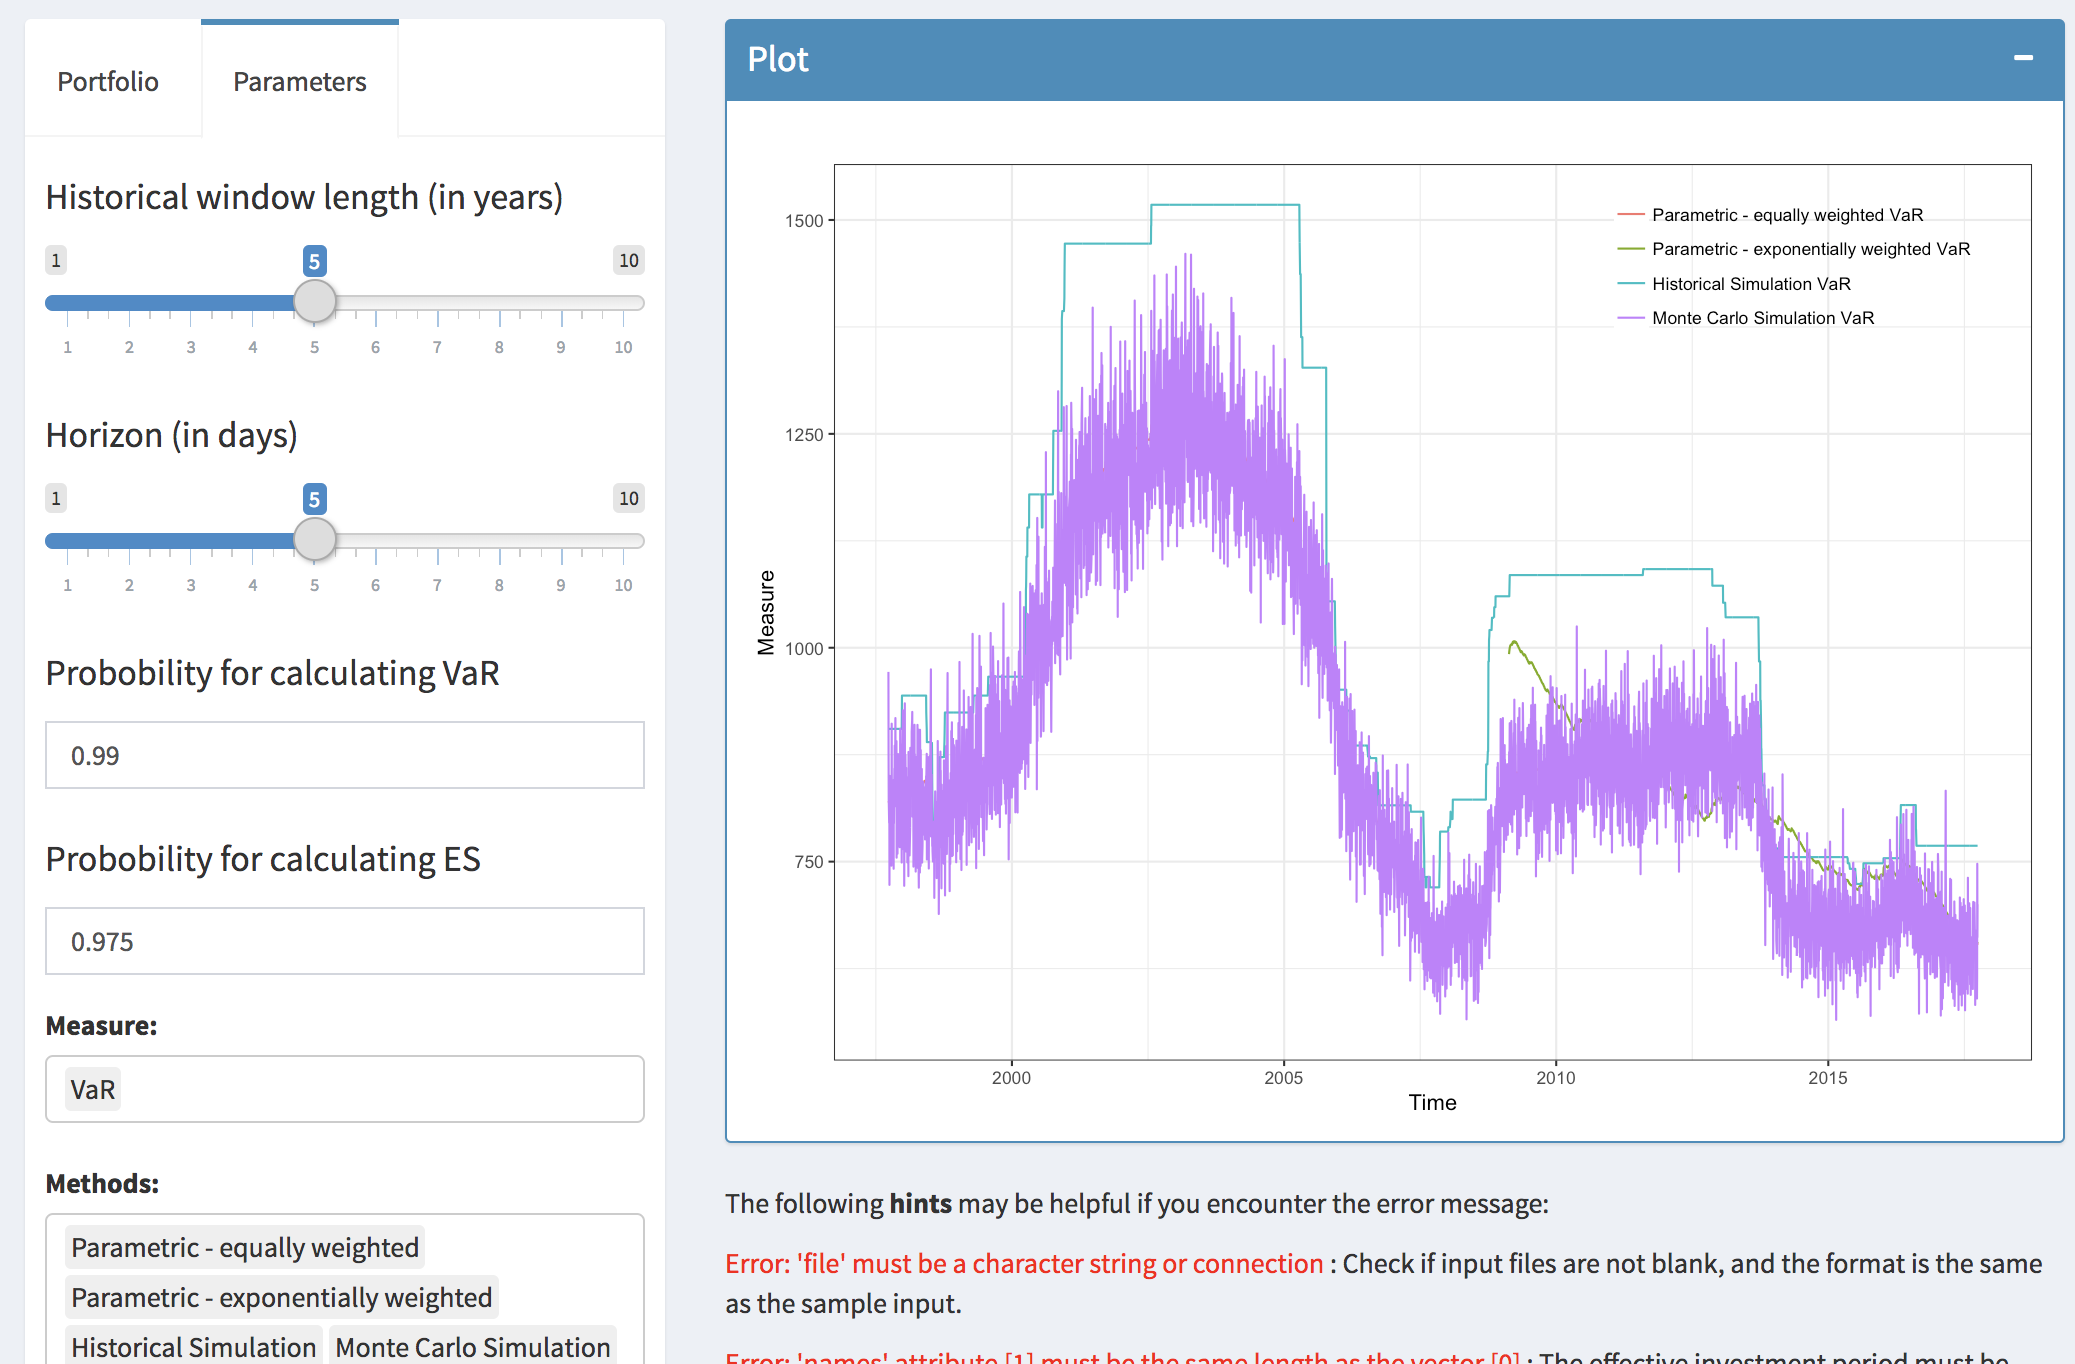
\includegraphics[width=0.49\textwidth]{fig/assvar.png}}
    \subfigure[Assignment ES]{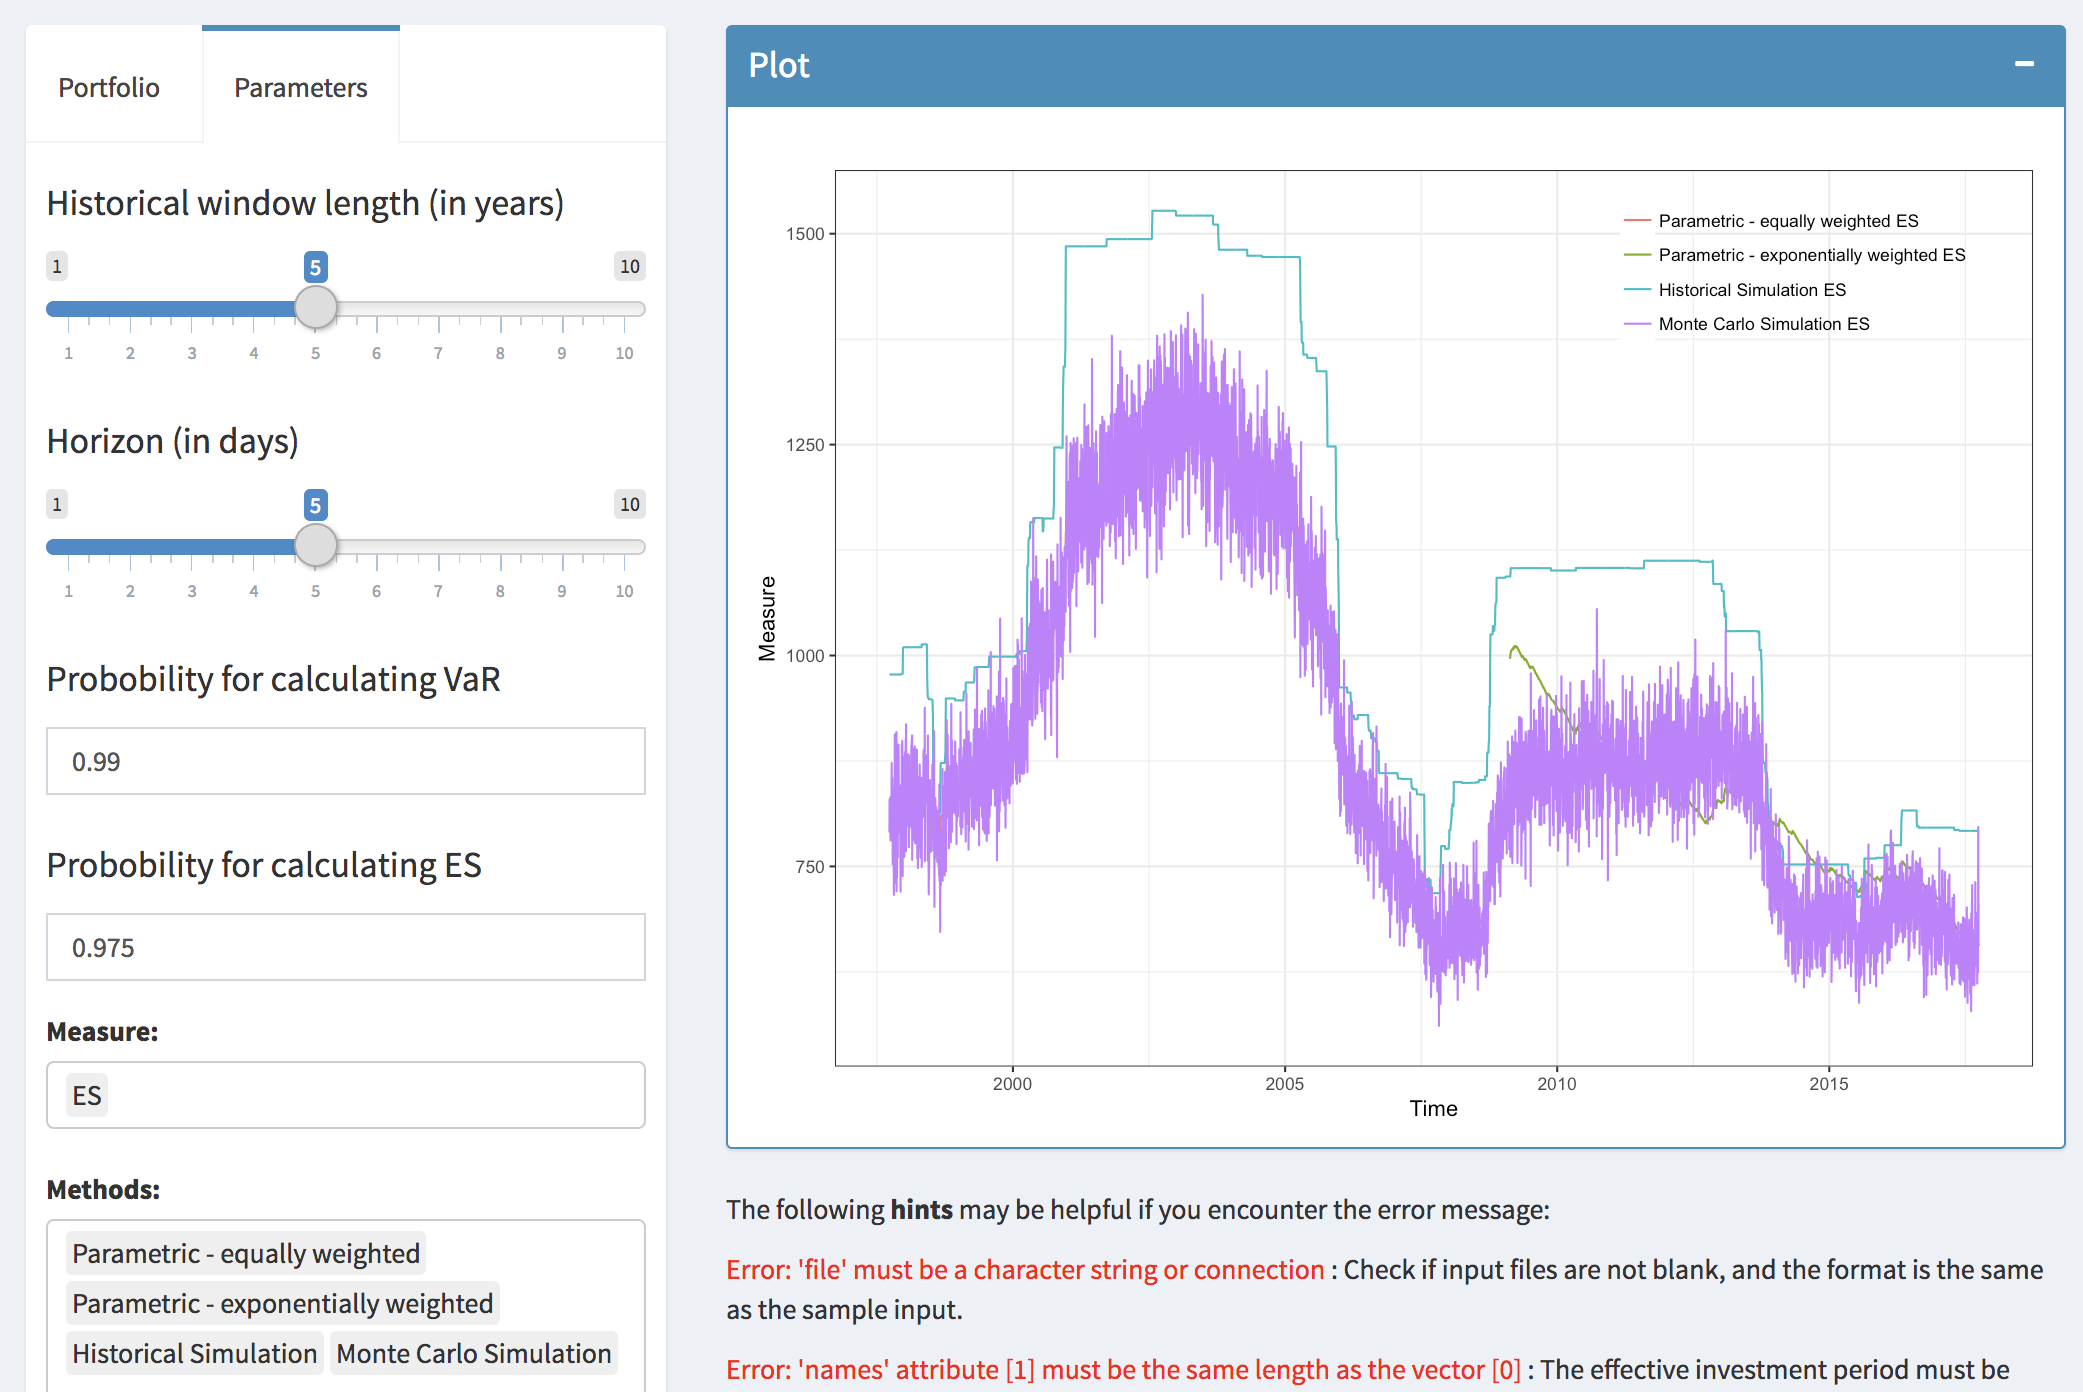
\includegraphics[width=0.49\textwidth]{fig/asses.png}}
    \caption{Result comparison with assignments}
    \label{fig:results:vg:loss}
    \end{figure}
    
    
As the result is the same as solution, we further look at backtesting results about the exceptions. We compare the equally weighted method with exponentially weighted method, exponentially weighted method with historical method,  historical method with Monte Carlo simulation (which is not covered in the assignment). Here are the results:

    \begin{figure}[!hbt]
    \center
    \subfigure[Equal v.s. exponential exceptions]{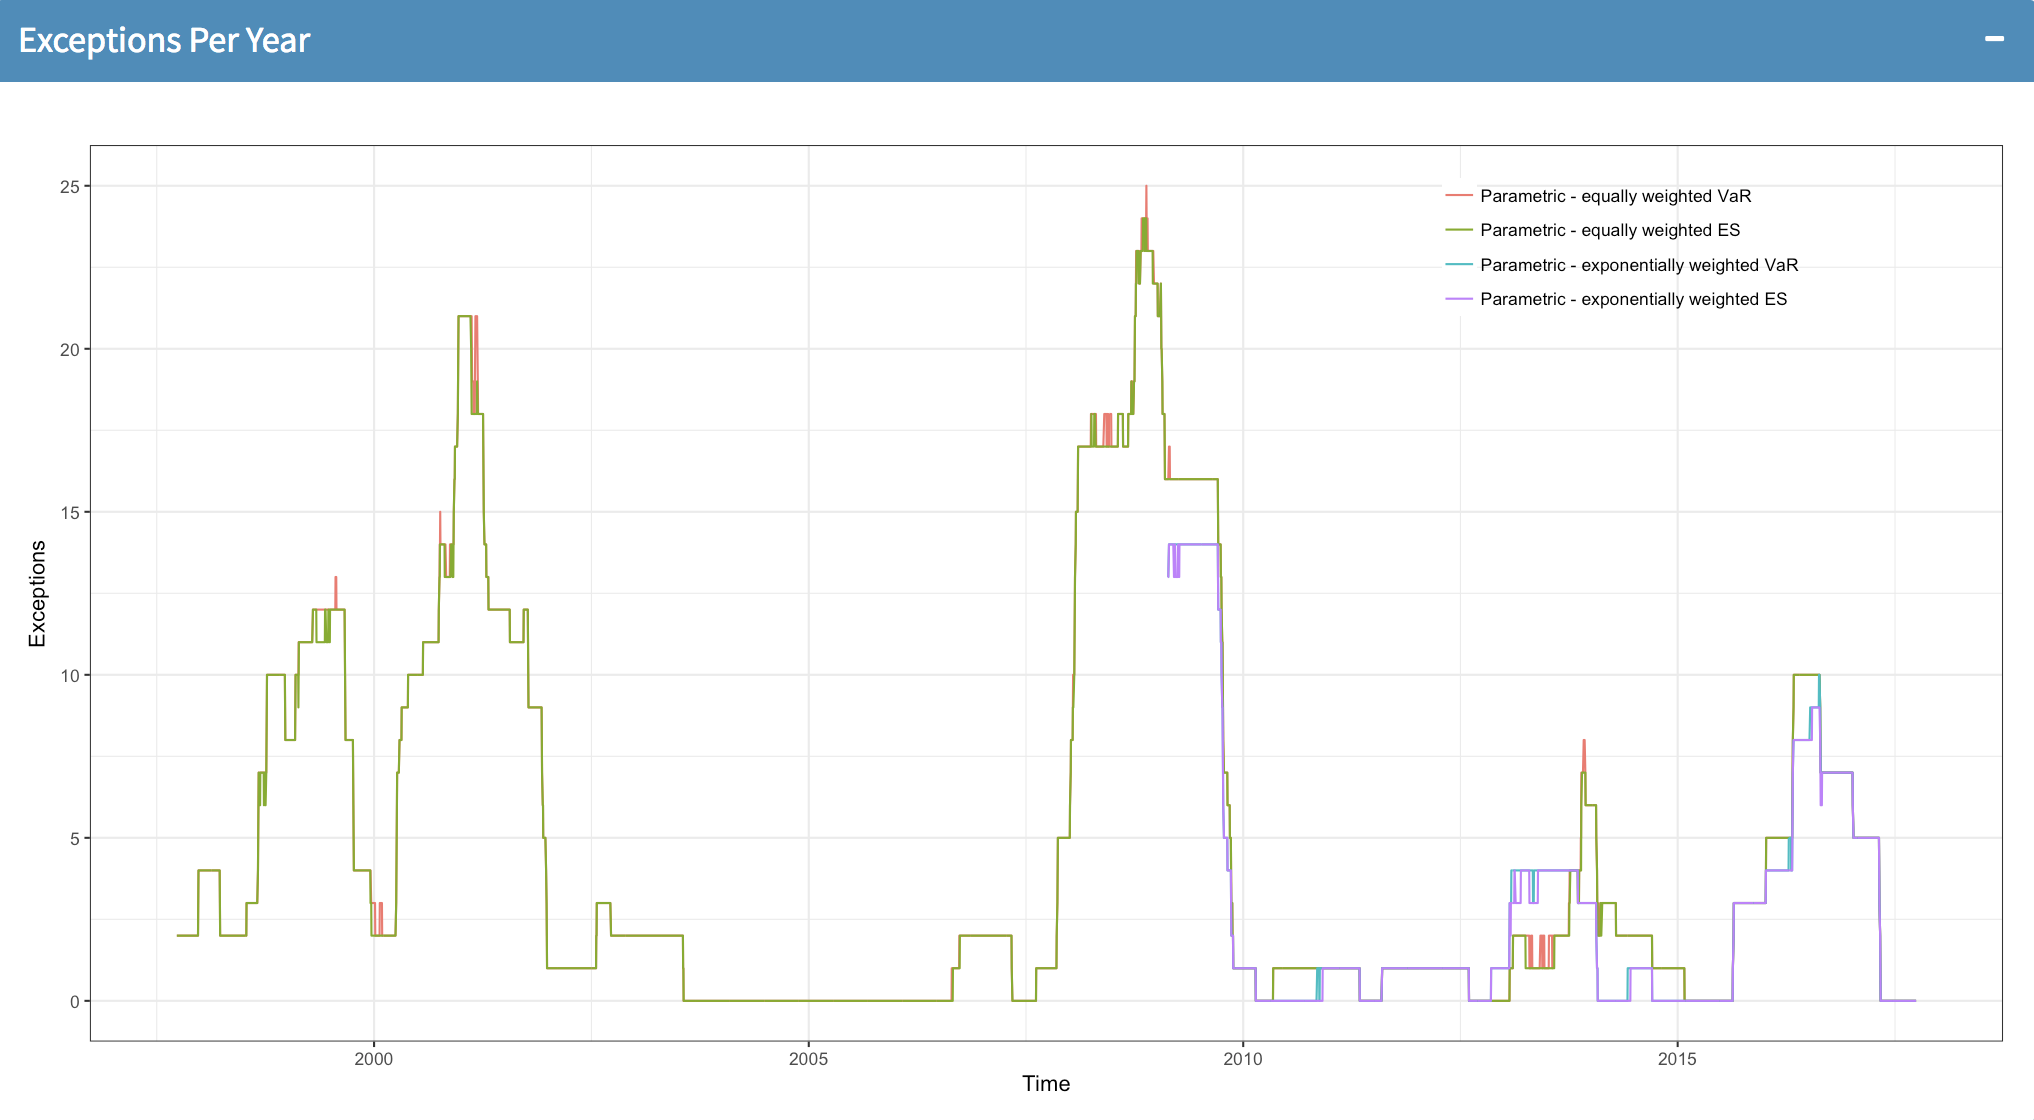
\includegraphics[width=0.49\textwidth]{fig/vs1.png}}
    \subfigure[Equal v.s. exponential  realized]{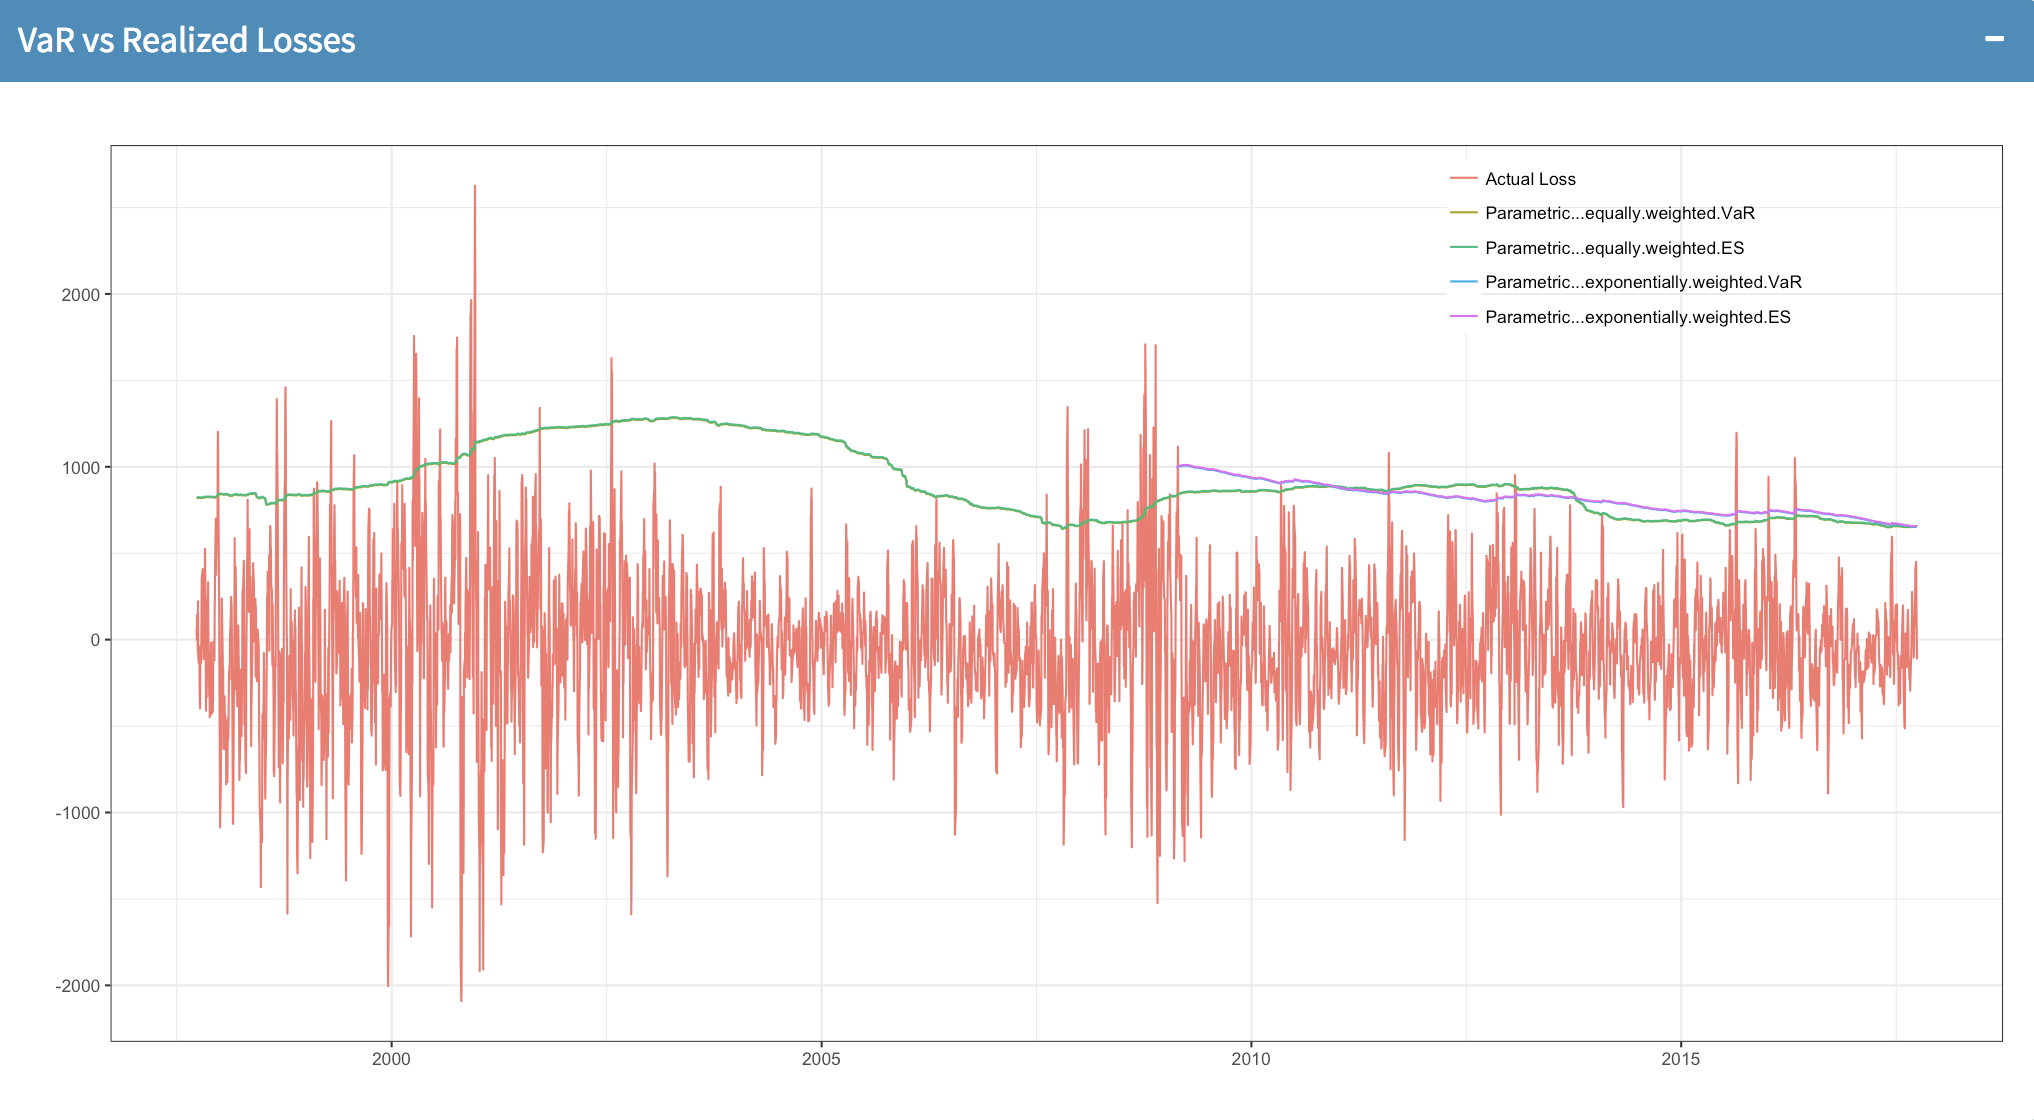
\includegraphics[width=0.49\textwidth]{fig/vs2.png}}
    \subfigure[Exponential v.s. historical exceptions]{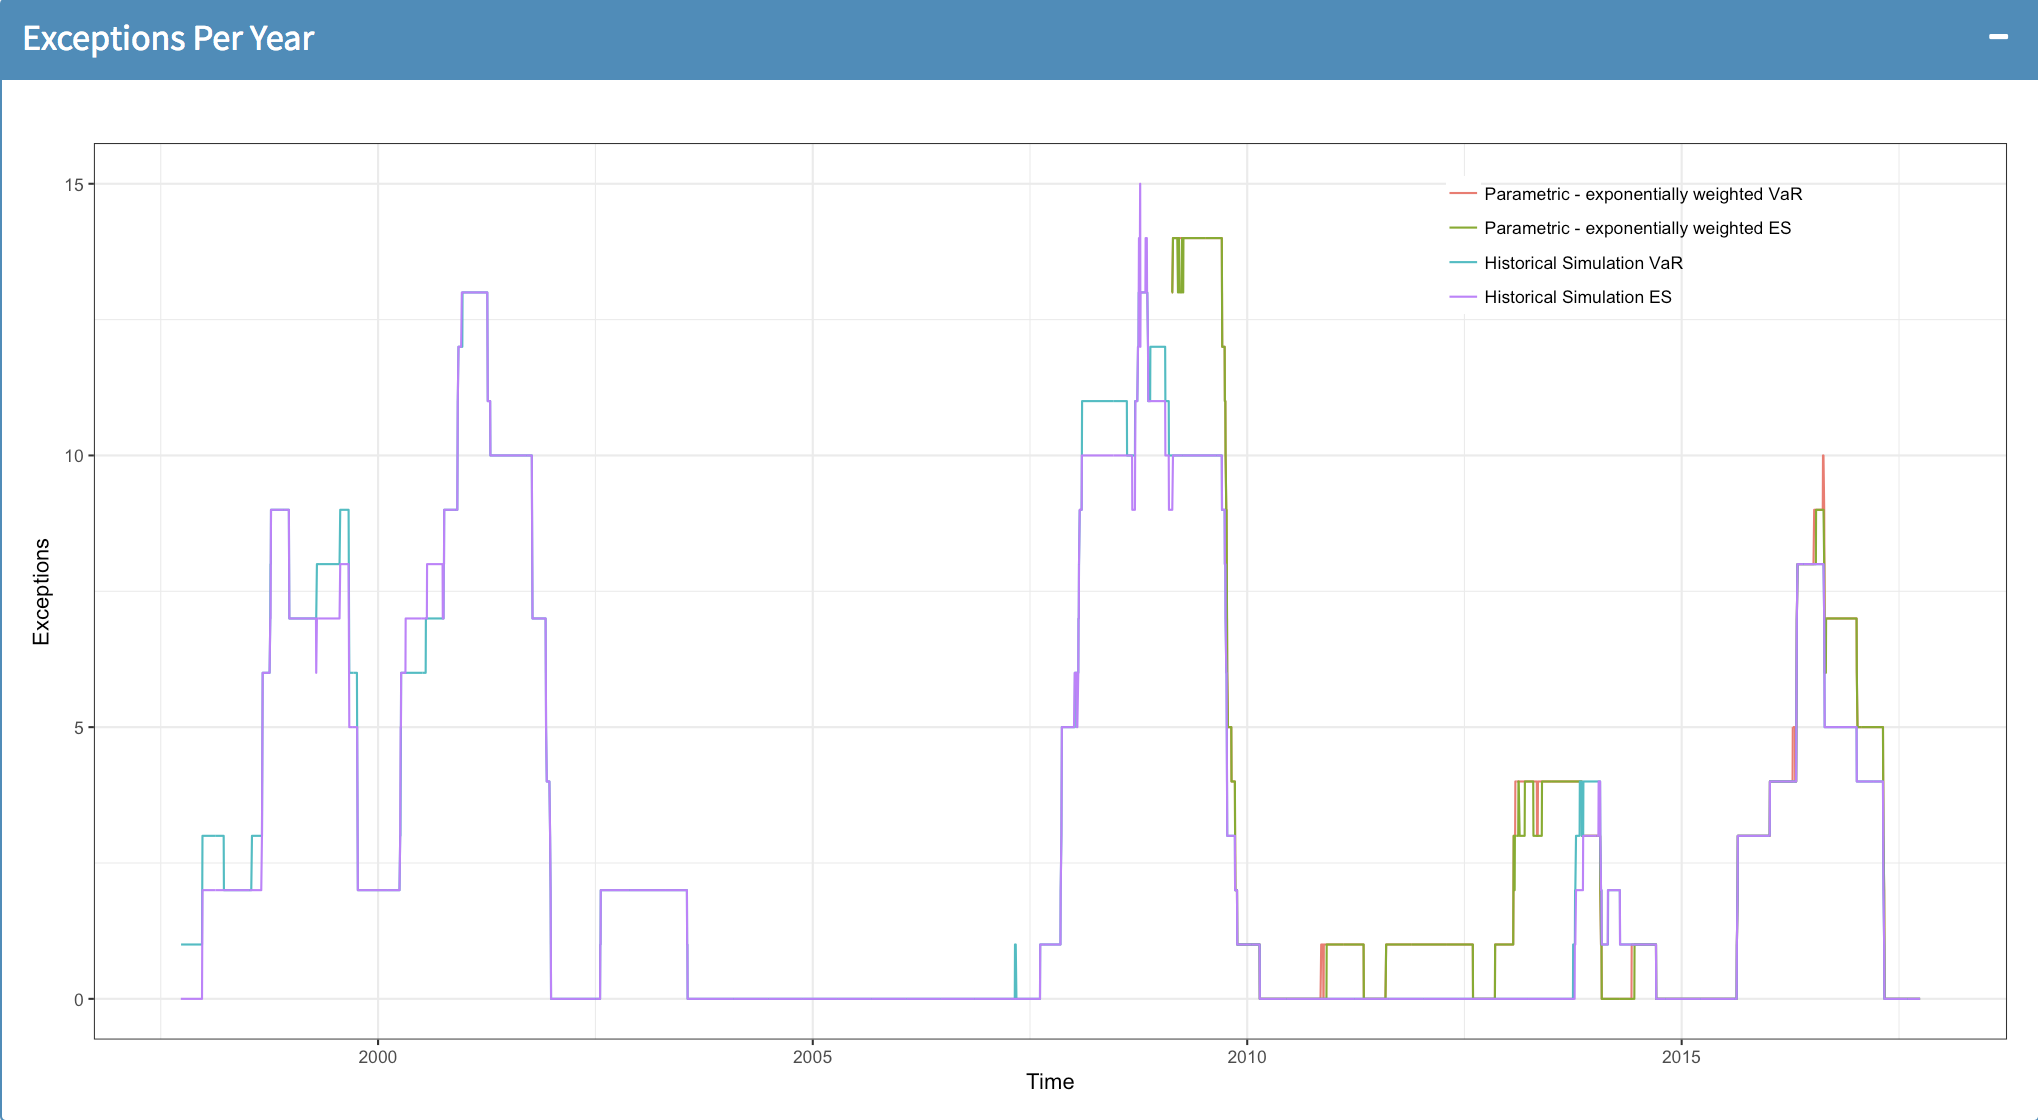
\includegraphics[width=0.49\textwidth]{fig/vs3.png}}
    \subfigure[Exponential v.s. historical  realized]{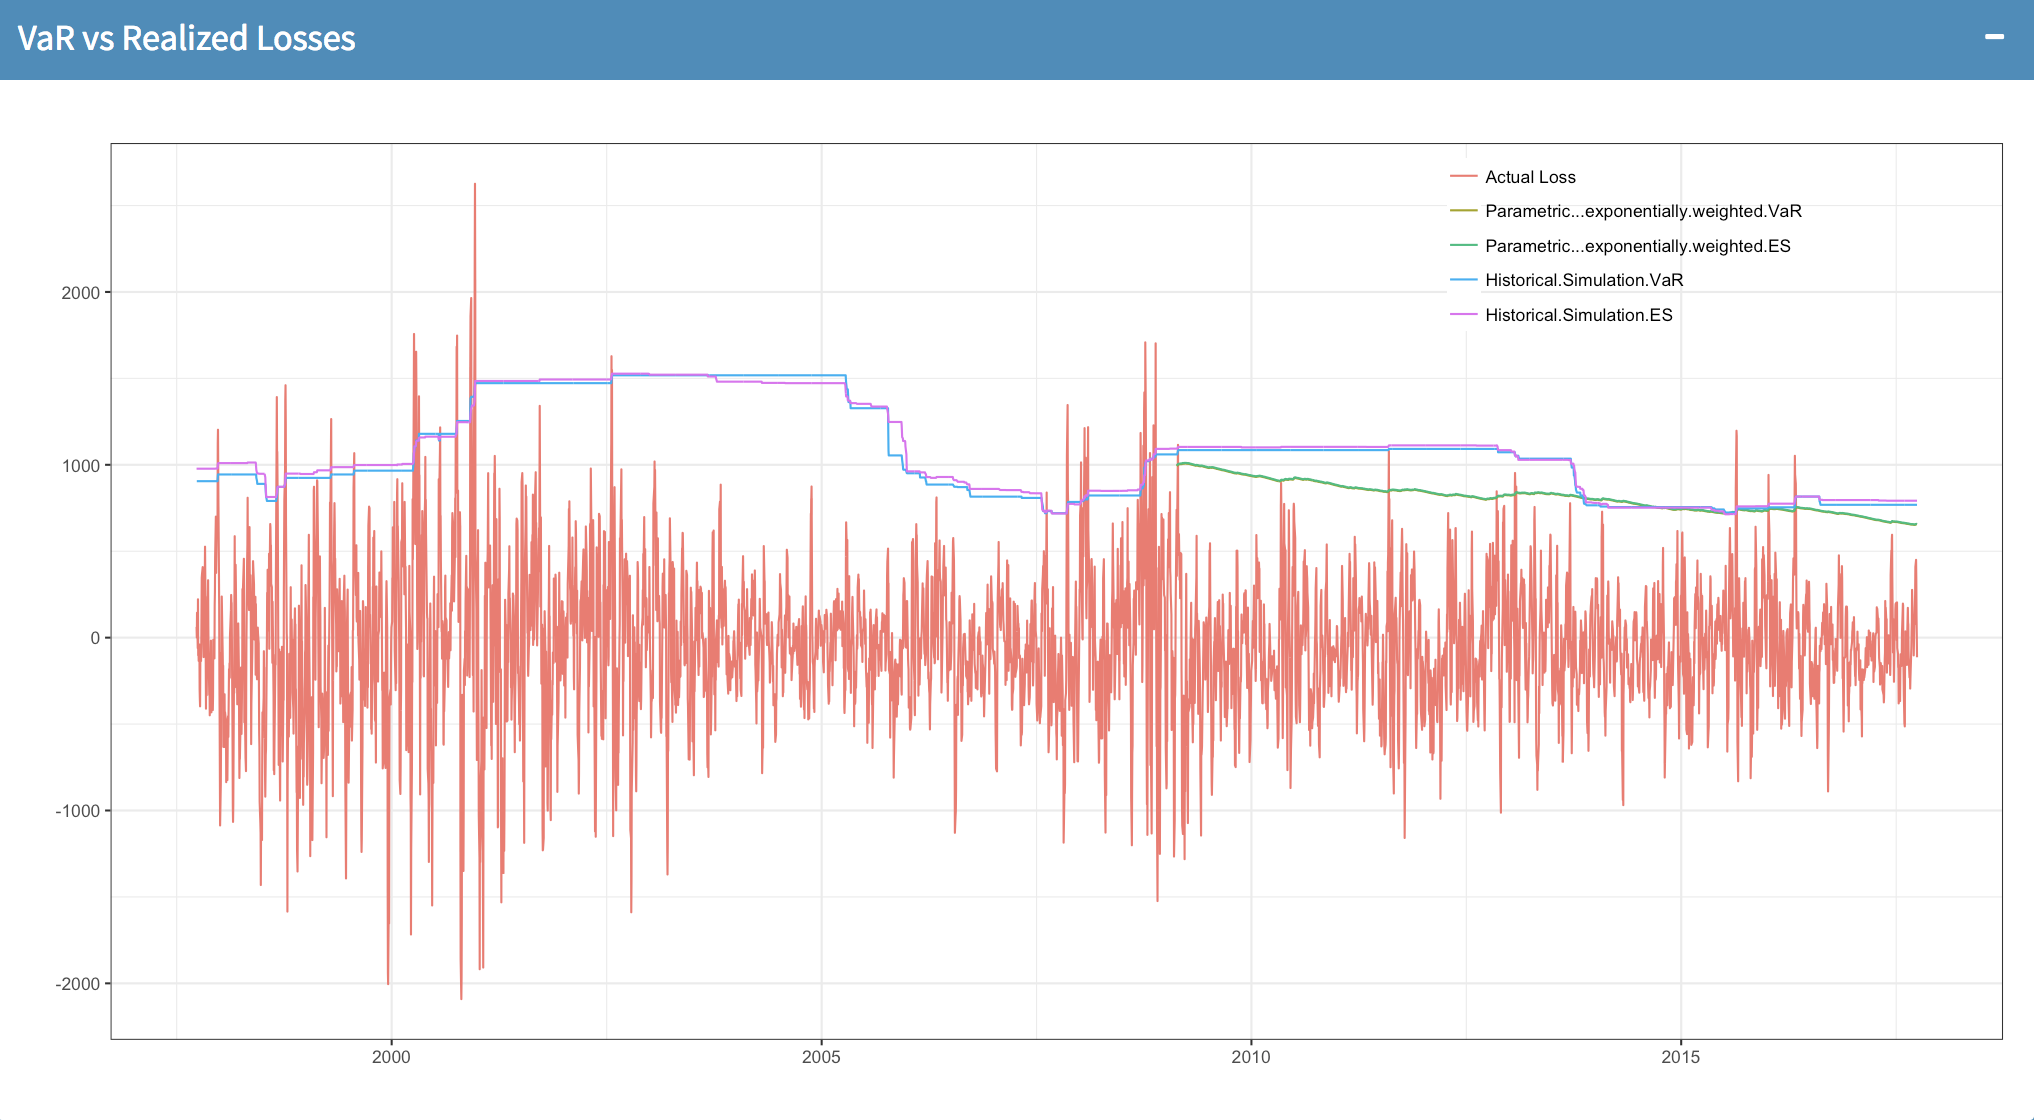
\includegraphics[width=0.49\textwidth]{fig/vs4.png}}   
    \subfigure[Historical v.s. MC exceptions]{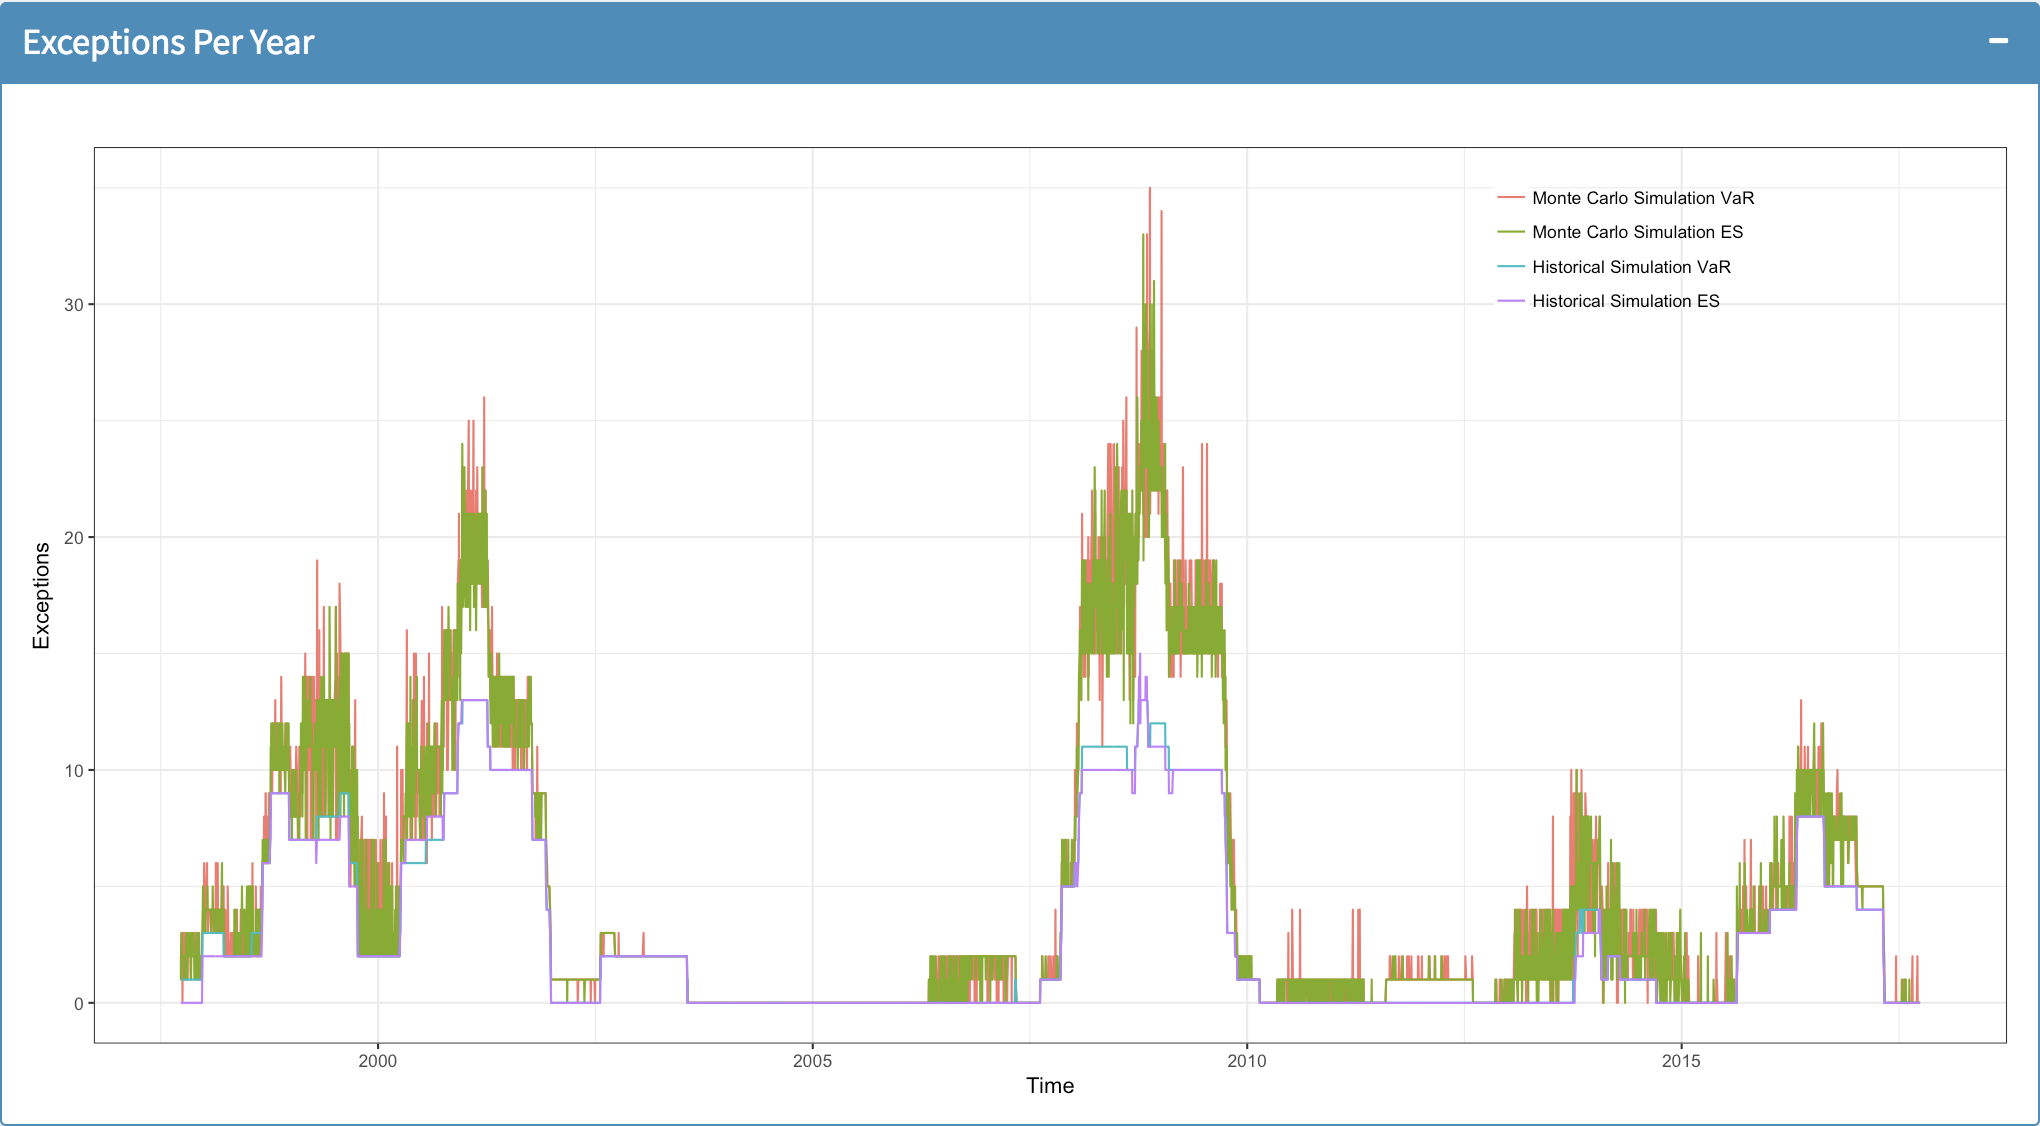
\includegraphics[width=0.49\textwidth]{fig/vs5.png}}
    \subfigure[Historical v.s. MC  realized]{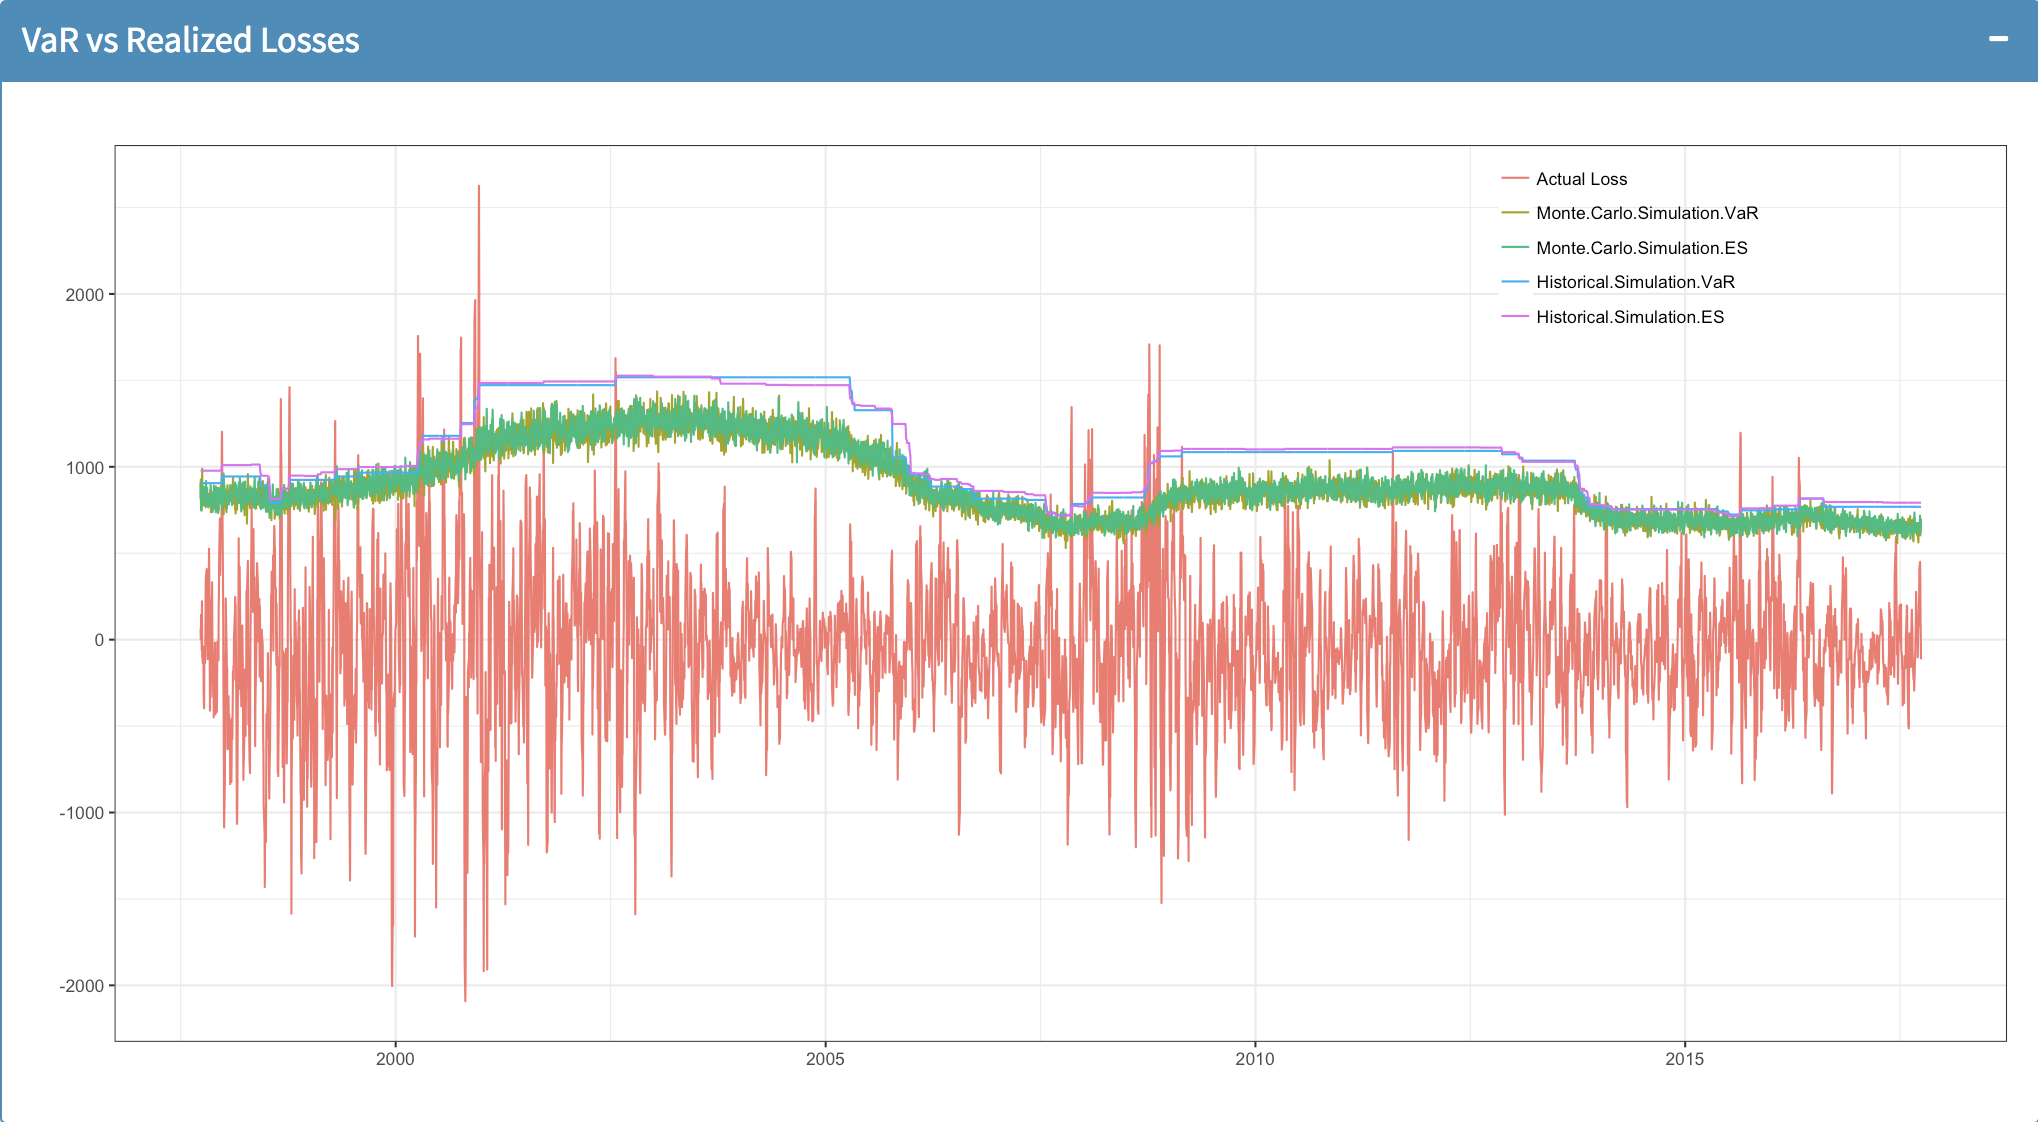
\includegraphics[width=0.49\textwidth]{fig/vs6.png}}
    \caption{Exceptions and realized comparison}
    \label{fig:results:vg:loss2}
    \end{figure}
    
We observe periods of time when there are no exceptions, and periods of time with a substantial number of exceptions.
Actual losses cluster.
Exceptions start occurring when volatility increases (as indicated by the range of the jumps in actual losses). The VaR starts to rise, but doesn’t rise fast enough to account for the increased market volatility. The VaR then falls when the volatility drops, but takes a long time to deflate to the new market behavior. 
The exponential weighting tends to yield fewer exceptions. Presumably, it is reacting to changes in volatility faster so the VaR is more realistic. 

Because sampling is from GBM distribution, Monte Carlo result behaves similar to equal weighted.

We then use a real to life example for furthering understand the result. The portfolio is combined with stocks AAPL, BBBY, CA, DISCA, EBAY, GOOG, INTC. Since MC behaves like parametric, we mainly focus on the difference between parametric and historical method.

    \begin{figure}[!hbt]
    \center
    \subfigure[Example risk measure]{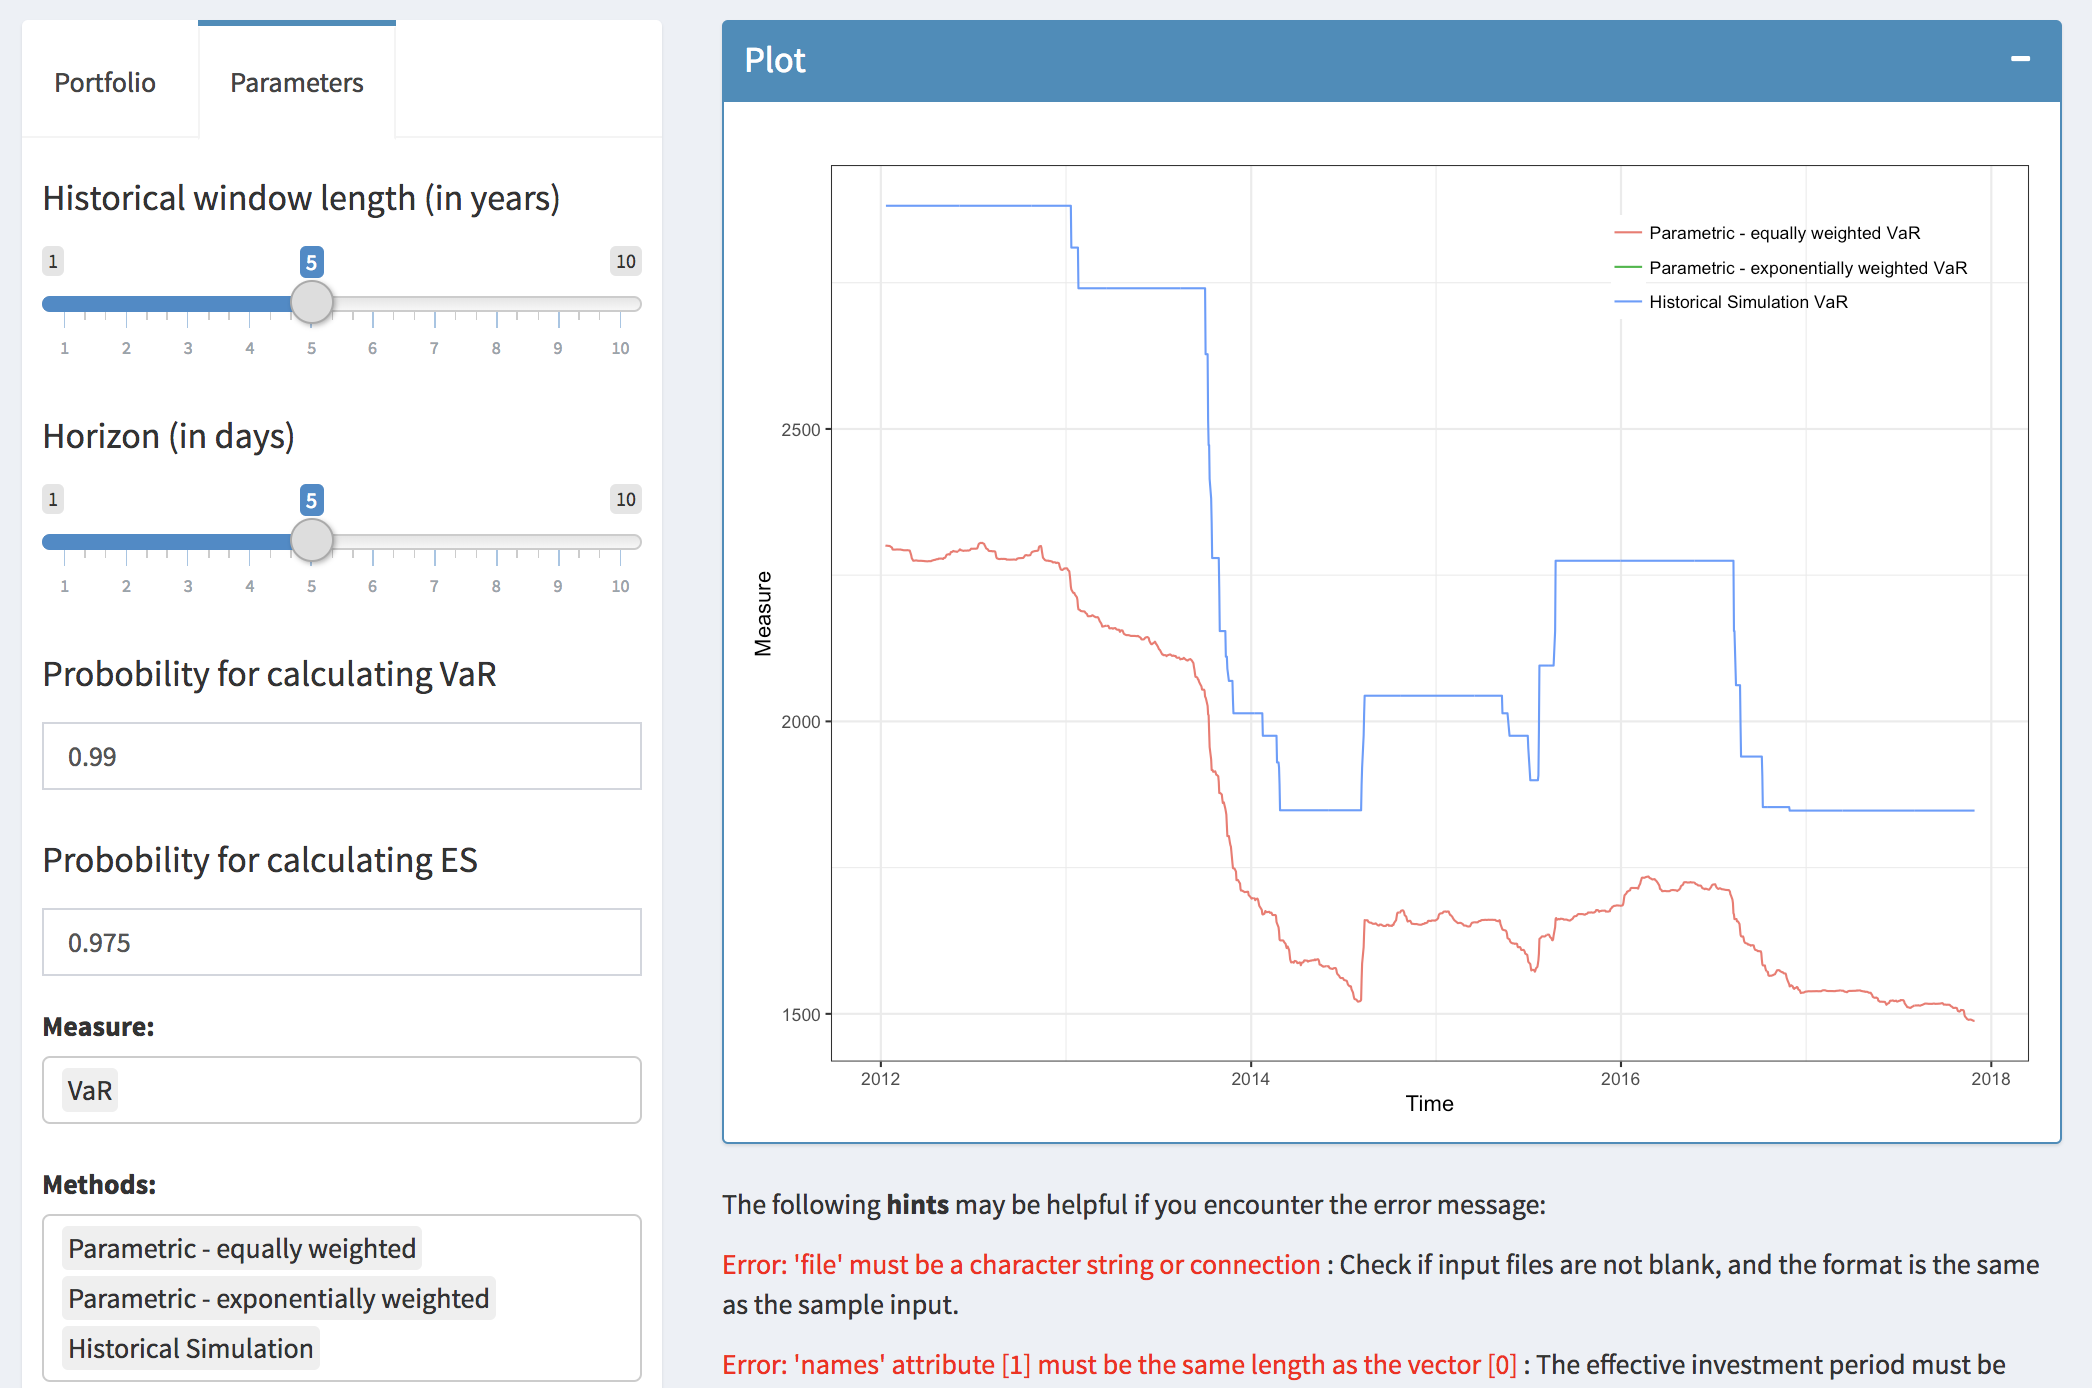
\includegraphics[width=0.7\textwidth]{fig/vs7.png}}
    \subfigure[Example exceptions]{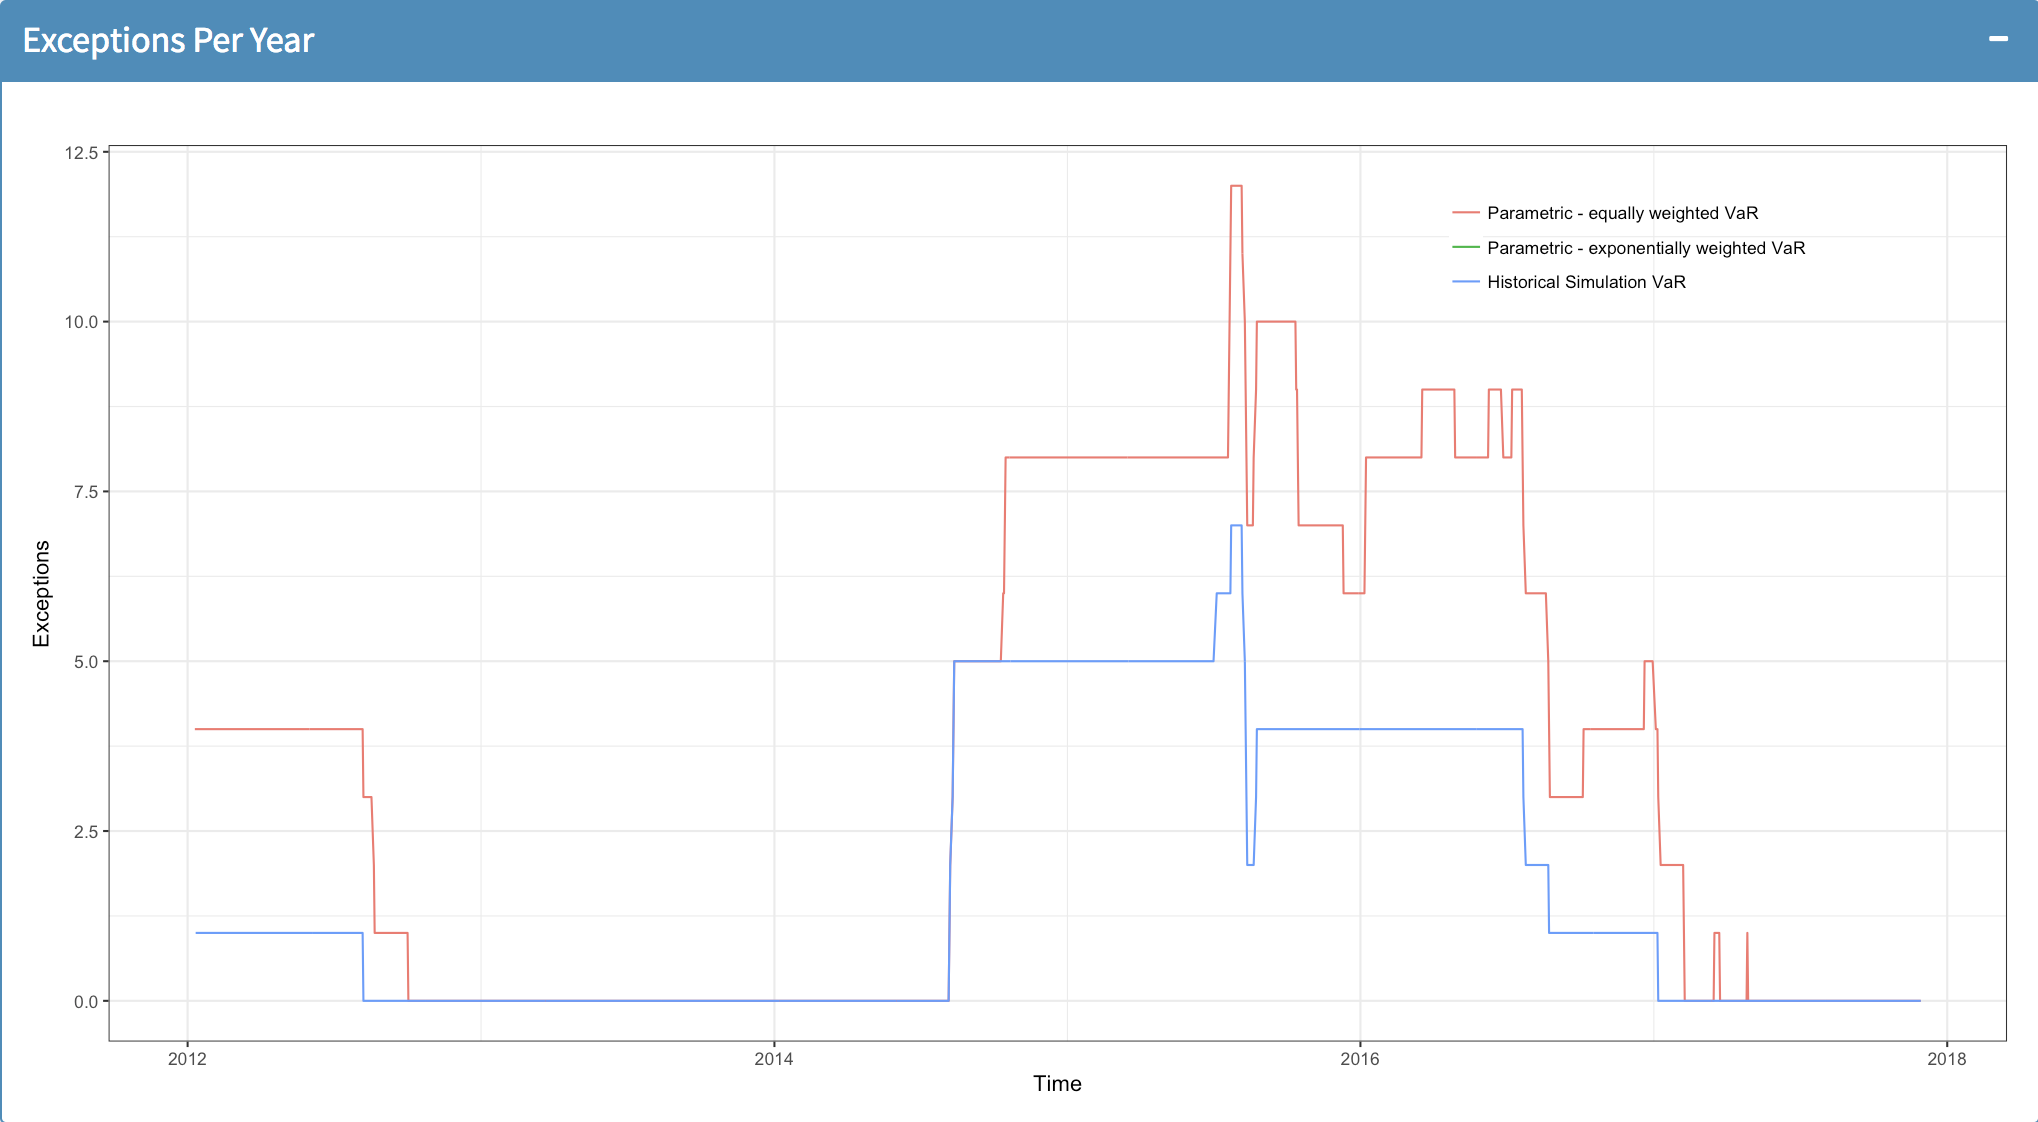
\includegraphics[width=0.49\textwidth]{fig/vs8.png}}
    \subfigure[Example realized]{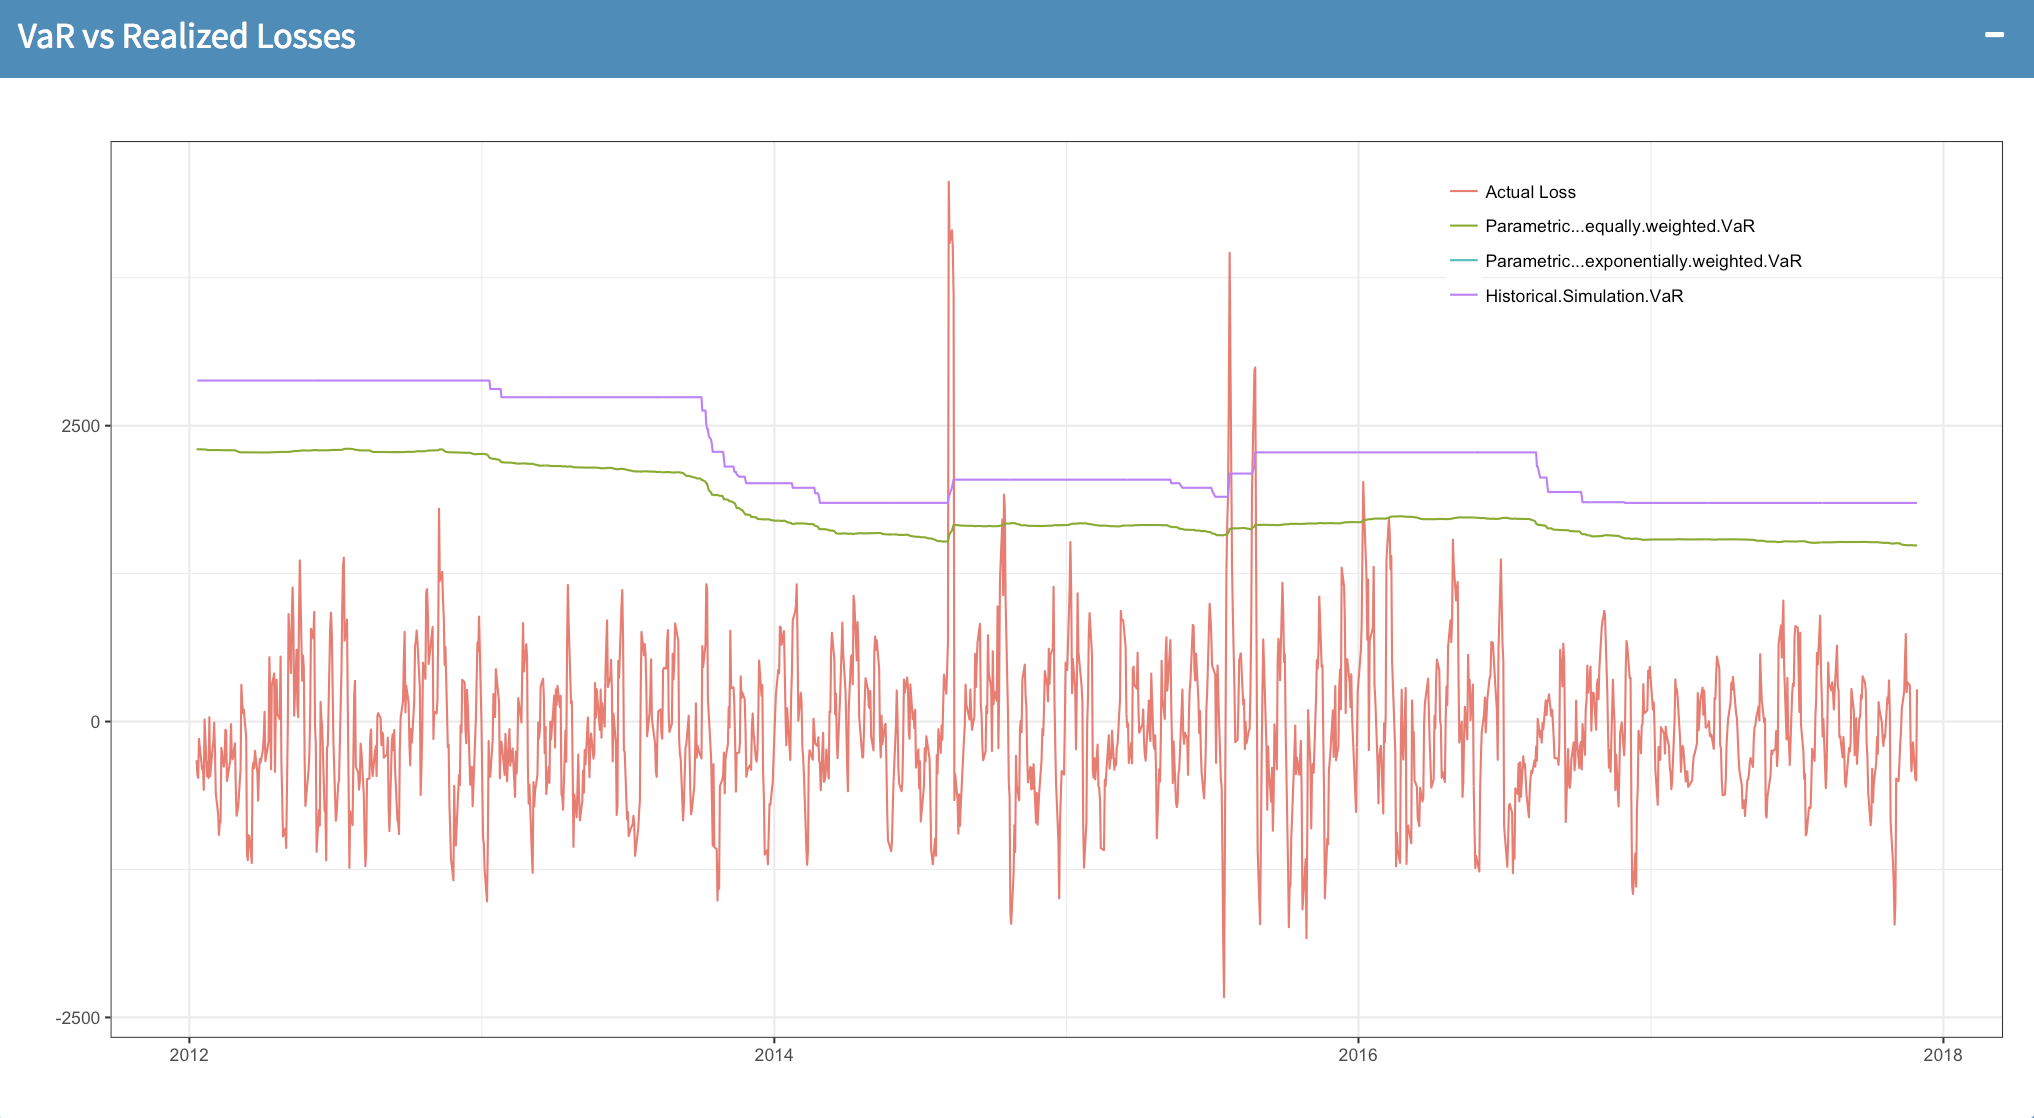
\includegraphics[width=0.49\textwidth]{fig/vs9.png}}
    \caption{Practical example for comparing parametric and historical method}
    \label{fig:results:vg:loss2}
    \end{figure}
    
The example shows that historical method is far more superior than parametric one, which also matches the fact that in real work, historical method is most frequently used. We should reconsider the usage of GBM.
    

%%%%%%%%%%%%%%%%%%%%%%%%%%%%%%%%%%%%%%%%%%%%%%

\begingroup
\renewcommand{\clearpage}{}
\chapter{Conclusions and Recommendations}
\label{chap:cr}
\endgroup

We first need to point out that GBM hypothesis is not so practical in the real life. To historical method,
it is very dependent on the historical data set, having difficulty handling shifts that take place during our sample period, making no allowance for plausible events that might occur, but did not actually occur, in our sample period.

The average exception is around 2.52, which is good, meaning that our system do have practical meanings. Moreover, if you run our system, you'll find it very pleasant for visualization and data collecting.

I would recommend to include more elegant models into our model to enhance the efficiency.


\appendix
\renewcommand\theequation{\Alph{chapter}--\arabic{equation}}
\renewcommand\thefigure{\Alph{chapter}--\arabic{figure}}
\renewcommand\thetable{\Alph{chapter}--\arabic{table}}

%\include{readme}

% !TEX encoding = UTF-8 Unicode
\chapter{R Code}
\label{app:code}

%%%%%%%%%%%%%%%%%%%%%%%%%%

\begin{spacing}{1}
\section{cal\_measure.R}
\label{sec:code:st}
\begin{lstlisting}
# price: current position
# s0: initial position
# windowLen: window length (in year). Default: 5 year window
# (windowLenDays <- windowLen * 252)
# horizonDays (in day). Default: 5 day horizon
# (horizon <- horizonDays / 252)



# CALIBRATION
# window
window_calibrate <- function(price, windowLen, horizonDays) {
  horizon <- horizonDays / 252
  windowLenDays <- windowLen * 252
  logreturn <- -diff(log(price), horizonDays)
  
  result <- NULL
  samplemu <- rollapply(logreturn, windowLenDays, mean)
  samplesig <- rollapply(logreturn, windowLenDays, sd)
  sig <- samplesig / sqrt(horizon)
  mu <- samplemu / horizon + sig ** 2/2

  df <- list(mu = mu, sigma = sig)
  return(df)
}

# exponential
solve_lambda <- function(windowLenDays){
  result <- uniroot(function(o) {
    2 * (2 * o**(windowLenDays + 1) + o**(windowLenDays + 2) + o**windowLenDays - o)
  }, c(.5, 1))
  return(result$root)
}
weighted_calibrate <- function(price, windowLenDays, horizonDays){
  lambda <- solve_lambda(windowLenDays)
  horizon <- horizonDays / 252
  logreturn <- -diff(log(price), horizonDays)
  l <- length(logreturn)
  
  windowLen <- ceiling(log(0.01) / log(lambda))
  if (windowLen > 5000) {windowLen = 5000}

  coef <- lambda ** seq(0, windowLen-1)
  weights <- coef / sum(coef)
  
  sigmu <- NULL
  if (l < windowLen) {return(NULL)}
  for (i in 1:(l - windowLen + 1)){
      mubar <- sum(weights * logreturn[i:(i + windowLen - 1)])
      varbar <- sum(weights * (logreturn[i:(i + windowLen - 1)]) ** 2) - mubar ** 2
      sigbar <- sqrt(varbar)
      sig <- sigbar / sqrt(horizon)
      mu <- mubar / horizon + sig ** 2/2
      temp <- c(sig, mu)
      sigmu <- rbind(sigmu, temp)
  }
   
  df <- list(mu = sigmu[,2], sigma = sigmu[,1])
  return(df)
}

# PARAMETRIC MEASURE
gbmVaR <- function(s0, mu, sigma, horizon, VaRp) {
  gbm <- s0 - s0 * exp(sigma * sqrt(horizon) * 
    qnorm(1 - VaRp) + (mu - sigma^2/2) * horizon)
  return(gbm)
}


gbmES <- function(s0, mu, sigma, horizon, ESp) {
  es <- s0 * (1 - exp(mu * horizon)/(1 - ESp) *
    pnorm(qnorm(1 - ESp) - sqrt(horizon) * sigma))
  return(es)
}

# HISTORIC SIMULATION
historical_VaR <- function(price, s0, windowLenDays, VaRp, horizonDays) {
  rtn <- -diff(log(price), horizonDays)
  mtm <- s0 * exp(rtn)
  pnl <- s0 - mtm

  VaR <- NULL
  if (length(mtm) < windowLenDays) {return(NULL)}
  for (i in 1:(length(mtm) - windowLenDays)){
    VaR[i] <- quantile(pnl[i:(i + windowLenDays)], VaRp, na.rm = TRUE)
  }
  return(VaR)
}

historical_ES <- function(price, s0, windowLenDays, ESp, horizonDays){
  rtn <- -diff(log(price), horizonDays)
  mtm <- s0 * exp(rtn)

  ES <- NULL
  if (length(mtm) < windowLenDays) {return(NULL)}
  for (i in 1:(length(mtm) - windowLenDays + 1)){
    Extreme <- quantile(mtm[i:(i + windowLenDays - 1)], 1 - ESp, na.rm = T)
    set <- mtm[i:(i + windowLenDays - 1)]
    ES[i] <- s0 - mean(set[set <= Extreme])
  }
  return(ES)
}

# MONTE CARLO
Monte_VaR <- function(s0, mu, sigma, VaRp, horizon, npaths){
  MCVaR <- vector()
  l <- length(mu)
  
  for (j in 1:l){
    pnl <- NULL
    for (i in 1:npaths){
      c <- rnorm(1,0,sqrt(horizon))
      temp <- s0 * exp((mu[j] - sigma[j] ** 2 / 2) * horizon + sigma[j] * c)
      pnl <- c(pnl, s0 - temp)
    }
    MCVaR <- c(MCVaR, quantile(pnl, VaRp, na.rm = T))
  }
  return(MCVaR)
}

Monte_ES <- function(s0, mu, sigma, ESp, horizon, npaths){
  MCES <- vector()
  l <- length(mu)
  
  for (j in 1:l){
    pnl <- NULL
    for (i in 1:npaths){
      c <- rnorm(1,0,sqrt(horizon))
      temp <- s0 * exp((mu[j] - sigma[j] ** 2 / 2) * horizon + sigma[j] * c)
      pnl <- c(pnl, s0 - temp)
    }
    temp <- pnl[pnl > quantile(pnl, ESp, na.rm = T)]
    ESvalue <- mean(temp)
    MCES <- c(MCES, ESvalue)
  }
  return(MCES)  
}

# CALCULATION
cal_measure <- function(s0, price, windowLen, horizonDays, 
  method, measure, npaths, VaRp, ESp, data) {
  windowLenDays <- windowLen * 252
  horizon <- horizonDays / 252

  # Choose method
  ## Parametric - equally weighted
  if (method == "Parametric - equally weighted") {
    if (measure == "VaR") {
      return(gbmVaR(s0, data$WindowMean, data$WindowSD, horizon, VaRp))
    }
    else {
      if (measure == "ES") {
        return(gbmES(s0, data$WindowMean, data$WindowSD, horizon, ESp))
      }
    }
  }

  ## Parametric - exponentially weighted
  else if (method == "Parametric - exponentially weighted") {
    if (measure == "VaR") {
      return(gbmVaR(s0, data$ExponentialMean, data$ExponentialSD , horizon, VaRp))
    }
    else {
      if (measure == "ES") {
        return(gbmES(s0, data$ExponentialMean, data$ExponentialSD, horizon, ESp))}
    }
  }

  ## Historical Simulation
  else if (method == "Historical Simulation") {
    if (measure == "VaR") {
      return(historical_VaR(price,s0,windowLenDays,VaRp,horizonDays))
    }
    else {
      if (measure == "ES") {
        return(historical_ES(price,s0,windowLenDays,ESp,horizonDays))
      }
    }
  }

  ## Monte Carlo Simulation
  else if (method == "Monte Carlo Simulation") {
    if (measure == "VaR") {
      return(Monte_VaR(s0, data$WindowMean, data$WindowSD, VaRp, horizon, npaths))
    }
    else {
      if (measure == "ES") {
        return(Monte_ES(s0, data$WindowMean, data$WindowSD, ESp, horizon, npaths))
      }
    }
  }
}
\end{lstlisting}
\end{spacing}


%%%%%%%%%%%%%%%%%%%%%%%%%%

\newpage
\begin{spacing}{1}
\section{ui.R}
\label{sec:code:nn}
\begin{lstlisting}
# Dashboard UI
library(shinydashboard)

shinyUI(
  dashboardPage(
    skin = 'blue',

    # # # # # header & navbar
    dashboardHeader(
      title = 'Risk System',
      tags$li(
        class = 'dropdown',
        tags$a(href = 'mailto:cd2904@columbia.edu, zs2331@columbia.edu', icon('envelope'))
      )
    ),

    # # # # # sidebar
    dashboardSidebar(
      sidebarMenu(id="tabs",
        menuItem("ReadMe", tabName = "readme", icon=icon("mortar-board")),
        menuItem("Plot", tabName="plot", icon=icon("line-chart"),
          menuSubItem("Risk Measure", tabName = "rm", icon = icon("angle-right"), selected=TRUE),
          menuSubItem("Back Testing", tabName = "bt", icon = icon("angle-right")),
          menuSubItem("Calibration", tabName = "cali", icon = icon("angle-right"))),
        menuItem("Table", tabName = "table", icon=icon("table"),
          menuSubItem("Source data", tabName = "sourcet", icon = icon("angle-right")),
          menuSubItem("Calibration", tabName = "calit", icon = icon("angle-right")),
          menuSubItem("Measure output", tabName = "measuret", icon = icon("angle-right")),
          menuSubItem("Exceptions", tabName = "exct", icon = icon("angle-right"))),
        menuItem("Option adjustment", tabName = "option", icon = icon("lightbulb-o"))
      )
    ),

    # # # # # main panel
    dashboardBody(
      tabItems(
        # Page 2-1
        tabItem(tabName = "rm",
          fluidRow(
            column(width = 4, 
              tabBox(width = NULL,
                tabPanel(h5("Portfolio"),
                  dateRangeInput("dates", start = "1992-09-24", label = h4("Investment period")),
                  hr(),
                  checkboxInput("checkfile", 
                    label = "Choice 1: upload file with close prices and volatility", value = TRUE),
                  fileInput("portfolio", h4("Position input")),
                  fileInput("investment", h4("Initial investment input")),
                  hr(),
                  checkboxInput("checkticker", 
                    label = "Choice 2: upload ticker name (available for stock only portfolio)", 
                    value = FALSE),
                  fileInput("tickerfile", h4("Ticker and investment input"))
                ),
                tabPanel(h5("Parameters"),
                  sliderInput("windowLen",
                    label = h4("Historical window length (in years)"),
                    min = 1, max = 10, value = 5),
                  sliderInput("horizonDays", label = h4("Horizon (in days)"),
                    min = 1, max = 10, value = 5),
                  numericInput("text1", 
                    label = h4("Probobility for calculating VaR"), value = 0.99),
                  numericInput("text2", 
                    label = h4("Probobility for calculating ES"), value = 0.975),
                  selectInput("measure", "Measure:", 
                    c("VaR", "ES"), selected = "VaR", multiple = TRUE, selectize = TRUE),
                  selectInput("method", "Methods:", c(
                    "Parametric - equally weighted", 
                    "Parametric - exponentially weighted",
                    "Historical Simulation", 
                    "Monte Carlo Simulation"), 
                  selected = "Parametric - equally weighted", multiple = TRUE, selectize = TRUE),
                  numericInput("npaths", label = h4("npaths"), value = 300),
                  submitButton("Submit")
                )
              )
            ),
            column(width = 8,
              box(width = NULL, plotOutput("measDataplot",height="500px"), collapsible = TRUE,
                title = "Plot", status = "primary", solidHeader = TRUE),
              p("The following", strong("hints"), "may be helpful if you encounter the error message:"),
              p(span("Error: 'file' must be a character string or connection", style = "color:red"),
                ": Check if input files are not blank, 
                and the format is the same as the sample input."),
              p(span("Error: 'names' attribute [1] must be the same length as the vector [0]", 
                style = "color:red"),
                ": The effective investment period must be greater than 0 day, 
                so change the investment period to see if it works."),
              p(span("Error: object 'variable' not found", 
                style = "color:red"),
                ": Check that method and measure input are not blank."),
              p(span("No plot output: ", 
                style = "color:red"),
                "Check if you have click the ", strong("submit "), "button.")
            )
          )
        ),
        # Page 2-3
        tabItem(tabName = "cali",
          box(width = NULL, plotOutput("caliDataplot1",height="500px"), collapsible = TRUE,
            title = "Mean Calibration Plot", status = "primary", solidHeader = TRUE),
          box(width = NULL, plotOutput("caliDataplot2",height="500px"), collapsible = TRUE,
            title = "Standard Calibration Plot", status = "primary", solidHeader = TRUE)
        ), 
        # Page 2-2
        tabItem(tabName = "bt",
          box(width = NULL, plotOutput("excDataplot1",height="500px"), collapsible = TRUE,
            title = "Exceptions Per Year", status = "primary", solidHeader = TRUE),
          box(width = NULL, plotOutput("excDataplot2",height="500px"), collapsible = TRUE,
            title = "VaR vs Realized Losses", status = "primary", solidHeader = TRUE)
        ), 
        # Page 3-1
        tabItem(tabName = "sourcet",
          box(width = NULL, status = "primary", solidHeader = TRUE, title="Source",  
            downloadButton('download_source', 'Download'), br(), br(),
            DT::dataTableOutput("ptfDatatable")
          )
        ),
        tabItem(tabName = "readme", includeMarkdown("../README.md")),
        # Page 3-2
        tabItem(tabName = "calit",
          box( width = NULL, status = "primary", solidHeader = TRUE, title="Calibration",
            downloadButton('download_cali', 'Download'), br(), br(),
            DT::dataTableOutput("caliDatatable")
          )
        ),
        # Page 3-3
        tabItem(tabName = "measuret",
          box(width = NULL, status = "primary", solidHeader = TRUE, title="Measurement", 
            downloadButton('download_measure', 'Download'), br(), br(),
            DT::dataTableOutput("measDatatable")
          )
        ),
        # Page 3-4
        tabItem(tabName = "exct",
          box(width = NULL, status = "primary", solidHeader = TRUE, title="Exceptions Per Year", 
            downloadButton('download_ex', 'Download'), br(), br(),
            DT::dataTableOutput("excDatatable")
          )
        ),
        tabItem(tabName = "option",
          fluidRow(
            column(width = 6, 
              box(width = NULL, solidHeader = TRUE, 
                title="When Portfolio has Option Positions", 
                fileInput("cvd", h4("Call volatility data")),
                fileInput("pvd", h4("Put volatility data")),
                fileInput("impl", h4("Implement")),
                numericInput("rf", label = h4("Risk free rate"), value = 0.05),
                numericInput("datenum", label = h4("Date (in numeric)"), value = 2)
              )
            ),
            column(6, 
              box(width = NULL, status = "primary", solidHeader = TRUE, 
                title="Adjusted VaR Output",
                verbatimTextOutput("optionData")
              )
            )
          )
        )
      )
    )
  )
)
\end{lstlisting}
\end{spacing}


%%%%%%%%%%%%%%%%%%%%%%%%%%

\newpage
\begin{spacing}{1}
\section{server.R}
\label{sec:code:vgg}
\begin{lstlisting}
# Dashboard Server
library(ggplot2)
library(dygraphs)
library(rowr)
library(DT)
library(zoo)
library(reshape2)


# user defined modules
source('../model/portfolio.R')
source("../model/cal_measure.R")
source("../model/option.R")

# server function
shinyServer(
  function(input, output) {
    # REACTIVES
    # ptfData: customize csv
    ptfData <- reactive({
      # use choice 1
      if (input$checkfile) {
        prices <- read.csv(input$portfolio$datapath)
        investment <- read.csv(input$investment$datapath)

        prices$Date <- as.Date(prices$Date, "%m/%d/%y")
        date_range <- c(as.Date(input$dates[1]), as.Date(input$dates[2]))
        start_date <- date_range[1]
        end_date <- date_range[2]
        prices <- prices[(prices$Date >= start_date) & (prices$Date <= end_date), ]
        init_prices <- prices[dim(prices)[1], ][-1]

        shares <- unlist(investment$amount / init_prices)
        portfolio <- 0
        for (i in 1:length(shares)) {
          portfolio <- portfolio + shares[i] * prices[, i+1]
        }
        prices$Portfolio <- portfolio
        prices$Date <- format(prices$Date)
        return(prices)
      } 
      # Warning: speed would be lower
      else if (input$checkticker) {
        stock_prices <- get_all_prices()
        position <- read.csv(input$tickerfile$datapath)
        date_range <- c(as.Date(input$dates[1]), as.Date(input$dates[2]))
        prices <- format_prices(stock_prices, position, date_range)
      
        # handle exception if no available data to form portfolio
        if (nrow(prices) == 0) {
          return(data.frame())
        }
      
        ptf <- format_portfolio(prices, position, date_range)
        return(ptf)
      }
    })

    # caliData: calibration of parametric mu and sigma 
    caliData <- reactive({
      ptf <- ptfData()
      price <- ptf$Portfolio
      windowLen <- input$windowLen
      windowLenDays <- windowLen * 252
      horizonDays <- input$horizonDays

      wincal <- window_calibrate(price, windowLen, horizonDays)
      expcal <- weighted_calibrate(price, windowLenDays, horizonDays)

      caliData <- cbind.fill(ptf$Date, wincal$mu, expcal$mu,
        wincal$sigma, expcal$sigma, fill = NA)
      names(caliData) <- c("Date", "WindowMean", "ExponentialMean", 
        "WindowSD", "ExponentialSD")
      caliData
      })

    # measData: gather all measures
    measData <- reactive({
      ptf <- ptfData()
      s0 <- ptf$Portfolio[dim(ptf)[1]]
      price <- ptf$Portfolio
      windowLen <- input$windowLen
      horizonDays <- input$horizonDays
      VaRp <- input$text1
      ESp <- input$text2
      method <- input$method
      measure <- input$measure
      npaths <- input$npaths
      caliData <- caliData()

      measData <- data.frame(Date = ptf$Date)
      names <- c()
      for (i in method) {
        for (j in measure) {
          measData <- cbind.fill(measData, 
            cal_measure(s0, price, windowLen, horizonDays, i, j, npaths, VaRp, ESp, caliData), fill = NA)
          names <- c(names, paste(i, j))
        }
      }
      names(measData) <- c("Date", names)
      measData
      })

    # excData: backtesting exceptions
    excData <- reactive({
      ptf <- ptfData()
      s0 <- ptf$Portfolio[dim(ptf)[1]]
      price <- ptf$Portfolio
      horizonDays <- input$horizonDays
      horizon <- horizonDays / 252
      nrows <- length(price)
      if (nrows < 252) {return(NULL)}

      ShareChange <- c(price[1:(nrows-horizonDays)] / price[(1+horizonDays):nrows], 
    rep(NA, horizonDays))

      measData <- measData()

      comparison <- data.frame(Date = ptf$Date)
      comparison <- cbind.fill(comparison, (s0 - ShareChange * s0), fill = NA)
      names(comparison) <- c("Date", "daysLoss")

      for (i in 2:(dim(measData)[2])) {
        measuredata <- measData[,i]
        exception <- c()
        for (i in 1:(nrows-252)) {
          exception <- c(exception, sum(comparison$daysLoss[i:(252+i-1)] >= measuredata[i]))
        }
        comparison <- cbind.fill(comparison, exception, fill = NA)
      }
      names(comparison) <- c("Date", "daysLoss", names(measData)[-1])
      comparison
    })

    # option
    optionData <- reactive({
      sp <- read.csv(input$portfolio$datapath)
      cv<- read.csv(input$cvd$datapath,header = T)
      cv[,2] <- cv[,2]/100
      pv<- read.csv(input$pvd$datapath,header = T)
      pv[,2] <- pv[,2]/100
      impl <- read.csv(input$impl$datapath)
      ci <- impl$index[1]
      pindex <- impl$index[2]
      siv <- c(5000, 5000)
      civ <- impl$invest[1]
      piv <- impl$invest[2]
      cm <- impl$maturity[1]
      pm <- impl$maturity[2]
      cs <- impl$strike[1]
      ps <- impl$strike[2]
      r <- input$rf
      w <- input$windowLen
      ho <- input$horizonDays
      vp <- input$text1
      np <- input$npaths
      da <- input$datenum
      combined_VaR(sp,cv,pv,ci,pindex,siv,civ,piv,cm,pm,cs,ps,r,da,vp,ho,w,np)
    })
    output$optionData <- renderPrint({ optionData() })
    # TABLES & DOWNLOADS
    # ptfData
    output$ptfDatatable <- DT::renderDataTable({
      df <- ptfData()
      for (i in names(df)[-1]) {
        df[,i] <- round(df[,i], 2)
      }
      DT::datatable(df, options = list(pageLength = 20))
    })
    output$download_source <- downloadHandler(
        filename = "source.csv",
        content = function(file) {write.csv(ptfData(), file, row.names = FALSE)}
    )

    # caliData
    output$caliDatatable <- DT::renderDataTable({
      df <- caliData()
      names(df) <- c("Date", "Window Mean", "Exponential Mean",
        "Window Standard Deviation", "Exponential Standard Deviation")
      for (i in names(df)[-1]) {
        df[,i] <- round(df[,i], 2)
      }
      DT::datatable(df, options = list(pageLength = 20))
    })

    output$download_cali <- downloadHandler(
        filename = "calibration.csv",
        content = function(file) {write.csv(caliData(), file, row.names = FALSE)}
    )

    # measData
    output$measDatatable <- renderDataTable({
      df <- measData()
      for (i in names(df)[-1]) {
        df[,i] <- round(df[,i], 2)
      }
      DT::datatable(df, options = list(pageLength = 20))
    })
    output$download_measure <- downloadHandler(
        filename = "measure.csv",
        content = function(file) {write.csv(measData(), file, row.names = FALSE)}
    )

    # excData
    output$excDatatable <- renderDataTable({
      df <- excData()
      for (i in names(df)[-1]) {
        df[,i] <- round(df[,i])
      }
      DT::datatable(df, options = list(pageLength = 20))
    })
    output$download_ex <- downloadHandler(
        filename = "exception.csv",
        content = function(file) {write.csv(excData(), file, row.names = FALSE)}
    )

    # PLOTS
    # caliData
    output$caliDataplot1 <- renderPlot({
      caliData <- caliData()[,1:3]
      # remove rows that have all NAs
      caliData <- caliData[!rowSums(!is.na(caliData[,-1])) == 0,]
      caliDataplot1 <- ggplot(melt(caliData, id.vars = "Date"), 
        aes(x = as.Date(Date), y = value, group = variable)) + 
        geom_line(aes(color = variable)) + 
        scale_color_discrete('', labels = c(
          "Window Mean", 
          "Exponential Mean")) +
        labs(title = '', x = 'Time', y = 'Mean calibration') +
        theme_bw() +
        theme(legend.position = c(0.9, 0.9), legend.background = element_blank())
        return(caliDataplot1)
    })
    output$caliDataplot2 <- renderPlot({
      caliData <- caliData()[,c(1,4,5)]
      # remove rows that have all NAs
      caliData <- caliData[!rowSums(!is.na(caliData[,-1])) == 0,]
      caliDataplot2 <- ggplot(melt(caliData, id.vars = "Date"), 
        aes(x = as.Date(Date), y = value, group = variable)) + 
        geom_line(aes(color = variable)) + 
        scale_color_discrete('', labels = c(
          "Window Standard Deviation", 
          "Exponential Standard Deviation")) +
        labs(title = '', x = 'Time', y = 'Standard deviation calibration') +
        theme_bw() +
        theme(legend.position = c(0.9, 0.9), legend.background = element_blank())
      return(caliDataplot2)
    })

    # measData
    output$measDataplot <- renderPlot({
      measData <- measData()
      # remove rows that have all NAs or NULLs
      if (dim(measData)[2] > 2) {
        measData <- measData[!rowSums(!is.na(measData[,-1])) == 0,]
      } else {
        measData <- na.omit(measData)
      }
      measDataplot <- ggplot(melt(measData, 
                  id.vars = "Date"), aes(x = as.Date(Date),
                                         y = value, group = variable)) + 
        geom_line(aes(color = variable)) + 
        scale_color_discrete('', labels = names(measData)[-1]) +
        labs(title = '', x = 'Time', y = 'Measure') +
        theme_bw() +
        theme(legend.position = c(0.8, 0.9), legend.background = element_blank())
      return(measDataplot)
    })

    # excData
    output$excDataplot1 <- renderPlot({
      comparison <- excData()
      # remove rows that have all NAs
      if (dim(comparison)[2] > 3) {
        comparison <- comparison[!rowSums(!is.na(comparison[,-c(1,2)])) == 0,]
      } else {
        comparison <- na.omit(comparison)
      }

      excDataplot1 <- ggplot(melt(comparison[,-2], 
                  id.vars = "Date"), aes(x = as.Date(Date),
                                         y = value, group = variable)) + 
        geom_line(aes(color = variable)) + 
        scale_color_discrete('', labels = names(comparison)[-c(1,2)]) +
        labs(title = '', x = 'Time', y = 'Exceptions') +
        theme_bw() +
        theme(legend.position = c(0.8, 0.9), legend.background = element_blank())
      return(excDataplot1)
    })
    output$excDataplot2 <- renderPlot({
      loss <- excData()[, c(1,2)]
      measData <- measData()[, -1]
      comparison <- cbind.fill(loss, measData, fill = NA)
      # remove rows that have all NAs
      if (dim(comparison)[2] > 3) {
        comparison <- comparison[!rowSums(!is.na(comparison[,-c(1,2)])) == 0,]
      } else {
        comparison <- na.omit(comparison)
      }

      excDataplot2 <- ggplot(melt(comparison, 
                  id.vars = "Date"), aes(x = as.Date(Date),
                                         y = value, group = variable)) + 
        geom_line(aes(color = variable)) + 
        scale_color_discrete('', labels = c("Actual Loss", names(comparison)[-c(1,2)])) +
        labs(title = '', x = '', y = '') +
        theme_bw() +
        theme(legend.position = c(0.8, 0.9), legend.background = element_blank())
      return(excDataplot2)
    }) 
})
\end{lstlisting}
\end{spacing}


%%%%%%%%%%%%%%%%%%%%%%%%%%%%%%%%%%%%%%%%%%%%%%

\backmatter

\bibliography{ref}
[1] Michel Crouhy, Dan Galai, Robert Mark. The Essentials of Risk Management, Second Edition. Book.


[2] John C. Hull. Risk Management and Financial Institutions (Wiley Finance) 4th Edition. Book.


[3] Robustness and sensitivity analysis of risk measurement procedures.Rama, Romain and Giacomo. SSRN.  
\url{https://papers.ssrn.com/sol3/papers.cfm?abstract_id=1086698}


[4]Model Validation, Harvey J. Stein. Model Validation Municipal Bonds. 2014


[5] \url{https://finance.zacks.com/common-risk-factors-returns-stocks-bonds-5893.html}




%%%%%%%%%%%%%%%%%%%%%%%%%%%%%%%%%%%%%%%%%%%%%%

\end{document}
